%% Преамбула TeX-файла

% 1. Стиль и язык
\documentclass[utf8x, 12pt]{G7-32} % Стиль (по умолчанию будет 14pt)

% Остальные стандартные настройки убраны в preamble.inc.tex.
\sloppy

% Настройки стиля ГОСТ 7-32
% Для начала определяем, хотим мы или нет, чтобы рисунки и таблицы нумеровались в пределах раздела, или нам нужна сквозная нумерация.
\EqInChapter % формулы будут нумероваться в пределах раздела
\TableInChapter % таблицы будут нумероваться в пределах раздела
\PicInChapter % рисунки будут нумероваться в пределах раздела

% Добавляем гипертекстовое оглавление в PDF
\usepackage[
bookmarks=true, colorlinks=true, unicode=true,
urlcolor=black,linkcolor=black, anchorcolor=black,
citecolor=black, menucolor=black, filecolor=black,
]{hyperref}

% Изменение начертания шрифта --- после чего выглядит таймсоподобно.
% apt-get install scalable-cyrfonts-tex

\IfFileExists{cyrtimes.sty}
    {
        %\usepackage{cyrtimespatched}
    }
    {
        % А если Times нету, то будет CM...
    }

\usepackage{graphicx}   % Пакет для включения рисунков

% С такими оно полями оно работает по-умолчанию:
% \RequirePackage[left=20mm,right=10mm,top=20mm,bottom=20mm,headsep=0pt]{geometry}
% Если вас тошнит от поля в 10мм --- увеличивайте до 20-ти, ну и про переплёт не забывайте:
\geometry{right=20mm}
\geometry{left=30mm}


% Пакет Tikz
\usepackage{tikz}
\usetikzlibrary{arrows,positioning,shadows}

% Произвольная нумерация списков.
\usepackage{enumerate}


% Настройки листингов.
% 8 Листинги

\usepackage{listings}

% Значения по умолчанию
\lstset{
  basicstyle= \footnotesize,
  breakatwhitespace=true,% разрыв строк только на whitespacce
  breaklines=true,       % переносить длинные строки
%   captionpos=b,          % подписи снизу -- вроде не надо
  inputencoding=koi8-r,
  numbers=left,          % нумерация слева
  numberstyle=\footnotesize,
  showspaces=false,      % показывать пробелы подчеркиваниями -- идиотизм 70-х годов
  showstringspaces=false,
  showtabs=false,        % и табы тоже
  stepnumber=1,
  tabsize=4,              % кому нужны табы по 8 символов?
  frame=single
}

% Стиль для псевдокода: строчки обычно короткие, поэтому размер шрифта побольше
\lstdefinestyle{pseudocode}{
  basicstyle=\small,
  keywordstyle=\color{black}\bfseries\underbar,
  language=Pseudocode,
  numberstyle=\footnotesize,
  commentstyle=\footnotesize\it
}

% Стиль для обычного кода: маленький шрифт
\lstdefinestyle{realcode}{
  basicstyle=\scriptsize,
  numberstyle=\footnotesize
}

% Стиль для коротких кусков обычного кода: средний шрифт
\lstdefinestyle{simplecode}{
  basicstyle=\footnotesize,
  numberstyle=\footnotesize
}

% Стиль для BNF
\lstdefinestyle{grammar}{
  basicstyle=\footnotesize,
  numberstyle=\footnotesize,
  stringstyle=\bfseries\ttfamily,
  language=BNF
}

% Определим свой язык для написания псевдокодов на основе Python
\lstdefinelanguage[]{Pseudocode}[]{Python}{
  morekeywords={each,empty,wait,do},% ключевые слова добавлять сюда
  morecomment=[s]{\{}{\}},% комменты {а-ля Pascal} смотрятся нагляднее
  literate=% а сюда добавлять операторы, которые хотите отображать как мат. символы
    {->}{\ensuremath{$\rightarrow$}~}2%
    {<-}{\ensuremath{$\leftarrow$}~}2%
    {:=}{\ensuremath{$\leftarrow$}~}2%
    {<--}{\ensuremath{$\Longleftarrow$}~}2%
}[keywords,comments]

% Свой язык для задания грамматик в BNF
\lstdefinelanguage[]{BNF}[]{}{
  morekeywords={},
  morecomment=[s]{@}{@},
  morestring=[b]",%
  literate=%
    {->}{\ensuremath{$\rightarrow$}~}2%
    {*}{\ensuremath{$^*$}~}2%
    {+}{\ensuremath{$^+$}~}2%
    {|}{\ensuremath{$|$}~}2%
}[keywords,comments,strings]

% Подписи к листингам на русском языке.
\renewcommand\lstlistingname{\cyr\CYRL\cyri\cyrs\cyrt\cyri\cyrn\cyrg}
\renewcommand\lstlistlistingname{\cyr\CYRL\cyri\cyrs\cyrt\cyri\cyrn\cyrg\cyri}


\usepackage{multirow}
\usepackage{amsmath}
\usepackage{longtable}

% Полезные макросы листингов.
% Любимые команды
\newcommand{\Code}[1]{\textbf{#1}}


\begin{document}

\frontmatter % выключает нумерацию ВСЕГО; здесь начинаются ненумерованные главы: реферат, введение, глоссарий, сокращения и прочее.

% Команды \breakingbeforechapters и \nonbreakingbeforechapters
% управляют разрывом страницы перед главами.
% По-умолчанию страница разрывается.

% \nobreakingbeforechapters
% \breakingbeforechapters

% Также можно использовать \Referat, как в оригинале
\begin{abstract}

\end{abstract}



\Defines
%\begin{description}
%\item[Распределённый] dddd
%\end{description}

x from~\cite{amd_pm_v2}.

\Abbreviations
%\begin{description}
%\item[АИС] lsdjfd
%\end{description}




\tableofcontents

\Introduction
Анализ сетевых пакетов всегда был и остается актуальной темой. Связано это с бурно растущей популярностью сети Интернет и стремительным ростом ее пользователей. Ранее анализ пакетов использовался для обнаружения проблем в сети и их дальнейшего устранения, а также широко использовался злоумышленниками для получения конфиденциальных данных.

Большинство имеющихся на данный момент разработок позволяют перехватывать сетевой трафик, сохранять его в каком-то виде, предоставляют способы для работы с сохраненными данными. К таким программам можно отнести все сетевые снифферы (tcpdump, Wireshark).

Технология глубого анализа является относительно новым направлением в сетевой отрасли. Ключевая идея состоит в том, чтобы анализировать не только данные канального, сетевого и транспортного уровней, но и данные остальных уровней сетевой модели OSI. Рост вычислительных мощностей современных компьютеров позволяет проводить такой анализ с высокой производительностью, что делает эту технологию привлекательной для использования в реальных системах, например:
\begin{itemize}
\item для блокировки определенного сетевого трафика;
\item для организации транспорта в сети путем изменения содержимого пакетов опеределенного типа;
\item для сбора статистических данных по каждому типу интересующего трафика;
\end{itemize}

В реальных системах сетевой сервис классификации трафика на основе технологии глубокого анализа может использоваться для пересылки более приоритетных пакетов (например, голоса) по более мощным линиям связи, или, например, для блокирови торрентов. Положиться на данные сетевого и транспортного уровня на 100\% нельзя, так как их легко можно подменить.

Разрабатываемый продукт акселерирован Intel DPDK, что позволит получить высокие показатели производительности, а также же дает преимущество перед существующими аналогами.


\mainmatter % это включает нумерацию глав и секций в документе ниже

\chapter{Аналитический раздел}
\label{cha:analysis}
\section{Анализ предметной области}
Сегодня невозможно представить человека без интернета и информационных технологий. Они прочно вошли в нашу жизнь, значительно упростив ее. С развитием информационных технологий нам становятся доступны новые инструменты, которые делают привычные нам процессы удобнее и быстрее, например: покупка товаров, оплата счетов, развлечения и многое другое. Наблюдается стремительный рост пользователей сети Интернет и объемов информации. Такое стремительное развитие в первую очередь отражается на интернет-провайдерах.

На рисунке~\ref{pic:user_connection_schema} представлена стандартная схема подключения пользователей к сети провайдера.
\begin{figure}
\centering
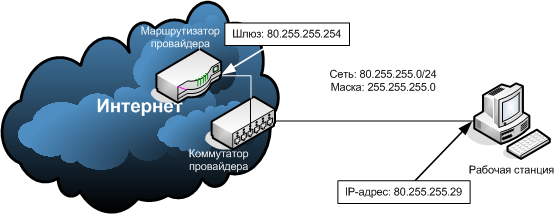
\includegraphics[scale=0.7]{pictures/user_connection_schema}
\caption{Подключение пользователя к сети Интернет}
\label{pic:user_connection_schema}
\end{figure}

В зависимости от видов предоставляемых услуг провайдеры деляется на:
\begin{itemize}
\item провайдеры доступа;
\item хостинг-провайдеры;
\itemмагистральные провайдеры;
\item канальные провайдеры;
\item провайдеры последней мили;
\end{itemize}

Независимо от того, к какой категории относятся провайдеры, они должны обеспечивать бесперебойную, надежную и высокоскоростную передачу данных абонентам. Данные задачи решаются такими методами, как:
\begin{itemize}
\item дублирование информации с целью минимизации расстояния между источником и потребителем;
\item увеличение пропускной способности каналов передачи данных;
\item приоритизация трафика и динамическое управление;
\end{itemize}

Подход, связанный с дублированием (репликацией) информации, активно используется на серверах баз данных. Является дорогим, так как требует дополнительных финансовых расходов, связанных с закупкой оборудования для хранения копий. Также требуется постоянная синхронизация между копиями для достижения консистентности данных.

Второй подход также связан с изменение сетевой инфраструктуры - модернизация каналов передачи данных с целью увеличения пропускной способность. Достигается за счет использования более быстрых способов коммутации, например оптоволокна. Аналогично первому подходу является дорогим.

Данная работа посвящена третьему подходу, связанному с приоритизацией и динамическим управлением трафиком. Основная идея заключается в классификации трафика по каким-то критериям и обработке разными способами. На рисунке \ref{pic:qos_simple_example} приведен пример использования классификации трафика для реализации QoS. Маршрутизатор 1 настроен таким образом, чтобы выделить до 5 МБит/с из доступных 10 МБит/с передаче потокового видео. Передаче данных по FTP разрешено использовать 2МБит/с, а HTTP и другому трафику до 3 МБит/с.
\begin{figure}
\centering
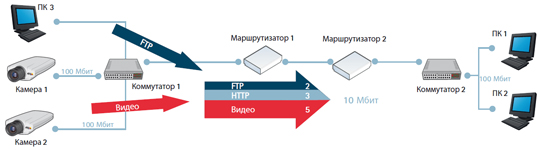
\includegraphics[scale=0.7]{pictures/qos_simple_example}
\caption{Пример динамического управления трафиком}
\label{pic:qos_simple_example}
\end{figure}

\subsection{Сетевая модель OSI и стек протоколов TCP/IP}
Сетевая модель OSI - базовая эталонная модель взаимодействия открытых систем. Назначение модели OSI состоит в обобщенном представлении средств сетевого взаимодействия, она разрабатывалась в качестве универсального языка сетевых специалистов, поэтому ее называют справочной моделью.

В связи с затянувшейся разработкой протоколов OSI, в настоящее время основным стеком протоколов является TCP/IP~\cite{modern_net}. Протоколы работают друг с другом в стеке - это означает, что протокол, располагающийся на уровне выше, работает
"поверх" нижнего, используя механизмы инкапсуляции. На рисунке~\ref{pic:model_osi_vs_tcpip} приведены обе модели, а также показаны их основные различия.
\begin{figure}[h]
\centering
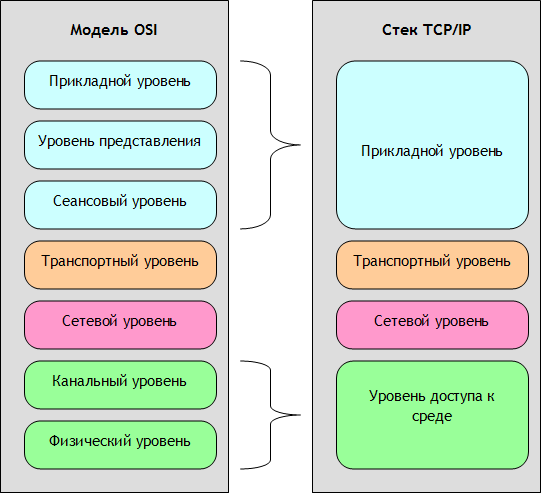
\includegraphics[scale=0.5]{pictures/model_osi_vs_tcpip}
\caption{Модель OSI и TCP/IP}
\label{pic:model_osi_vs_tcpip}
\end{figure}

На канальном уровне в большинстве сетей используется семейство технологий пакетной передачи данных Ethernet. В зависимости от скорости передачи данных, а также передающей среды, существует несколько вариантов технологии:
\begin{itemize}
\item ранние модификации Ethernet;
\item 10 МБит/с Ethernet;
\item Быстрый Ethernet (Fast Ethernet, 100 МБит/с);
\item Гигабитный Ethernet (Gigabit Ethernet, 1 ГБит/с);
\item 2.5 и 5-гигабитные варианты (NBASE-T, MGBASE-T);
\item 10-гигабитный Ethernet (10G Ethernet, 10 ГБит/с);
\item 40-гигабитный и 100-гигабитный Ethernet;
\end{itemize}

Разрабатываемый сетевой сервис будет работать только с Ethernet картами любых скоростей, при этом другие технологии канального уровня не поддерживаются.

\subsection{Технология DPI}
Анализ пакетов является важной задачей не только для классификации трафика, но и для всего функционирования сети. Любой сетевой коммутатор вынужден просматривать каждый пакет с целью изучения его mac-адреса отправителя и получателя. Эта информация нужна ему для того, что определить в какой выходной порт отправить пакет. Сетевые маршрутизаторы просматривают ip-адреса отправителя и получателя (если речь идет о TCP/IP сетях) и строят таблицы маршрутизации.

В наше время провайдеры сталкиваются с проблемами, которые не могут решиться только анализом заголовков пакетов, например:
\begin{itemize}
\item высокая загрузка канала к пользователю (скачивание BitTorrent);
\item высокая нагрузка на каналы провайдера (все пользователи скачивают BitTorrent);
\item большая часть пропускной способности занимается наименьшей частью наиболее активных абонентов;
\item атаки на оборудование, вирусы, боты;
\end{itemize}

Для решения всех этих проблем может применяться технология DPI - технология накопления статистических данных, проверки и фильтрации сетевых пакетов по их содержимому. Ключевая идея состоит в том, чтобы анализировать не только заголовки пакетов, такие как Ethernet, IP, TCP или UDP, но и остальные данные пакета с целью выявления определенных сигнатур или других особенностей, присущих искомому трафику. Самыми распространенными способами реализации DPI являются статический анализ и анализ косвенных признаков, присущих определенным протоколам. 

Система DPI, как правило, устанавливается на границе сети провайдера в разрыв существующих каналов, уходящих в пограничные маршрутизаторы, тем самым весь трафик, который покидает или входит в сеть оператора проходит через DPI, что дает возможность его мониторинга и контроля. В отдельных случаях можно устанавливать эту систему не на границе сети, а спускать ее ближе к конечным пользователям, но из экономических соображений так делают редко.

На рынке DPI есть модели от различных вендоров по различным ценам, все зависит от производительности и списка возможностей. В данной работе рассматривается чисто программная реализация технологии DPI под архитектуру процессоров x86\_64.


\section{QoS и DPI}
С точки зрения эксплуатации, провайдер может контролировать утилизацию подключенных через DPI каналов на уровне приложений. Раньше задача реализации QoS решалась исключительно средствами построения очередей на основании маркировки трафика служебными битами в заголовках IP, а также используя VLAN или MPLS метки, выделяя наиболее приоритетный трафик и гарантируя ему определенную пропускную способность в любой момент времени. При этом весь трафик домашних абонентов оставался без контроля, что давало возможность трафику BitTorrent забрать себе всю свободную полосу.

С использованием DPI у провайдера появляется возможность распределить канал между различными приложениями, так, например, можно разрешить в ночные часы BitTorrent с большей пропускной способностью, чем днем, когда в сети находится большое количество другого трафика.


\section{Межсетевой экран}
Межсетевой экран - комплекс аппаратных и программных средств в компьютерной сети, осуществляющий контроль и фильтрацию проходящих через него сетевых пакетов в соответствии с заданными правилами. Основной задачей сетевого экрана является защита сети или отдельных ее узлов от несанкционированного доступа, осуществление трансляции адресов - динамическую замену внутрисетевых (серых) адресов или портов на внешние, используемые за пределами локальной сети.

Различают следующие типы межсетевых экранов:
\begin{itemize}
\item управляемые коммутаторы (канальный уровень);
\item сетевые фильтры (сетевой уровень, анализ ip-адресов);
\item шлюзы сеансового уровня;
\item шлюз прикладного уровня (прокси-сервера);
\end{itemize}

В ядре Linux есть межсетевой экран под названием Netfilter, встроен в ядро с версии 2.4. Основным инструментов управления является Iptables - утилита командной строки, с ее помощью администраторы создают и изменяют правила, управляющие фильтрацией и перенаправлением пакетов.

В системе Netfilter пакеты пропускаются через цепочки. Цепочка является упорядоченным списком правил, а каждое правило может содержать критерии, действие или переход. Когда пакет проходит через цепочку, система по очереди проверяет, соответствует ли пакет всем критериям очередного правила, и если так, то выполняет действие. Набор критериев в системе Netfilter ограничен только заголовками протоколов и никак не учитывает остальную часть пакета, что является главным недостатком и не допускает использование Netfilter в сетях провайдера.

Существуют расширенные версии Netfilter, позволяющие выполнять более детальную проверку пакетов. Все они являются узкоспециализированными и реализуются, в основном, патчами ядра Linux, что предполагает перекомпиляцию самого ядра. Такое решение является непрактичным и используется редко.

Технология DPI идеально подходит для реализации функций межсетевого экрана, так как выполняет полный анализ пакета. Главным преимуществом является возможность контролировать информацию на прикладном уровне и классифицировать сотни протоколов без привязки к конкретному порту TCP или UDP. Благодаря этому можно, к примеру, блокировать Skype-трафик, а также любые виды SIP-телефонии.

Разрабатываемый сервис будет выполнять функции межсетевого экрана.


\section{Балансировка трафика}
Рано или поздно провайдер сталкивается с необходимостью распределять трафик по нескольким каналам, при этом необходимо, чтобы каждый канал использовался по максимуму. Распределение может осуществляться по разными критериям и разными способами в зависимости от организации внутренней сети провайдера и существующих маршрутов.

Одним из возможных вариантов организации внутренней сети провайдера является организация сети на основе MPLS и VLAN~\cite{modern_net}.

\subsection{MPLS сети}
Архитектура MPLS обеспечивает построение магистральных сетей, имеющих практически неограниченные возможности масштабирования, повышенную скорость обработки трафика и беспрецедентную гибкость с точки зрения организации дополнительных сервисов. Кроме того, технология MPLS позволяет интегрировать сети IP и ATM, за счет чего поставщики услуг могут не только сохранить средства, инвестированные в оборудование асинхронной передачи, но и извлечь дополнительную выгоду из совместного использования этих протоколов.

В основе MPLS лежит принцип обмена метками. Любой передаваемый пакет ассоциируется с тем или иным FEC, каждый из которых идентифицируется определенной меткой. Значение метки уникально лишь для участка пути между соседними узлами сети MPLS. Метка передается в составе любого пакета, причем способ ее привязки к пакету может быть различным. На рисунке~\ref{pic:mpls_label} показана структура метки.
\begin{figure}[h]
\centering
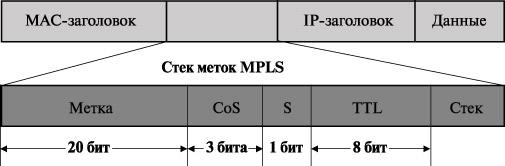
\includegraphics[scale=0.5]{pictures/mpls_label}
\caption{Структура MPLS метки}
\label{pic:mpls_label}
\end{figure}

Размер метки 4 байта. Она состоит из следующих полей:
\begin{itemize}
\item метка (LABEL), размер поля - 20 бит, используется для определения LSP;
\item класс сервиса (Class Of Service, CoS), размер поля - 3 бита, используется для реализации механизмов качества обслуживания и явного уведомления о перегрузке;
\item дно стека (Bottom Of Stack, S), размер поля - 1 бит, если флаг установлен, это означает, что данная метка является последней в стеке;
\item время жизни (Time To Live, TTL), размер поля - 8 бит, используется для предотвращения петель, как и в IP;
\end{itemize}

Распределение меток между LSR приводит к установлению внутри домена MPLS путей с коммутацией по меткам - LSP. Обмен метками между LSR осуществляется с использованием LDP, а также с помощью модифицированных версий других протоколов сигнализации в сети. Каждый маршрутизатор LSR содержит таблицу, которая ставит в соответствие паре "входной интерфейс, входная метка" тройку "префикс адреса получателя, выходной интерфейс, выходная метка". Получая пакет, LSR по номеру интерфейса, на который пришел пакет, и по значению метки определяет для него выходной интерфейс. Старое значение метки заменяется новым и пакет отправляется следующему устройству на пути LSP.

Вся операция требует лишь одноразовой идентификации значений полей в одной строке таблицы. Это занимает гораздо меньше времени, чем сравнение IP-адреса отправителя с наиболее длинным адресным префиксом в таблице маршрутизации, используемой при традиционном подходе.

Сеть MPLS делится на две функционально различные области - ядро и граничную область (рисунок~\ref{pic:mpls_net_example}). Ядро образуют устройства, минимальным требованием к которым является поддержка MPLS и участие в процессе маршрутизации трафика. Маршрутизаторы ядра занимаются только коммутацией. Все функции классификации пакетов по различным FEC, а также реализацию таких дополнительных сервисов, как фильтрация, явная маршрутизация, выравнивание нагрузки и управление трафиком, берут на себя граничные LSR.  В результате интенсивные вычисления приходятся на граничную область, а высокопроизводительная коммутация выполняется в ядре.
\begin{figure}
\centering
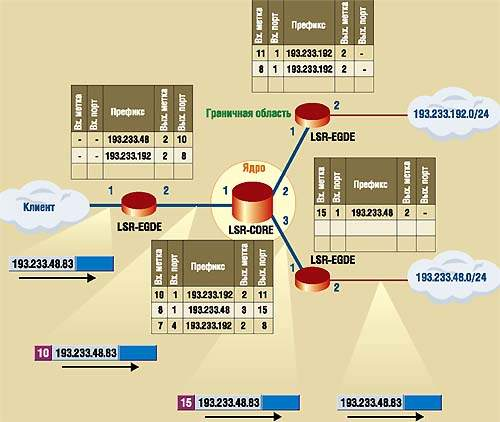
\includegraphics[scale=0.55]{pictures/mpls_net_example}
\caption{Схема коммутации MPLS}
\label{pic:mpls_net_example}
\end{figure}

На граничных маршрутизаторах может быть реализована классификация трафика с использованием технологии DPI. Такой подход придаст сети большую гибкость, гарантируя наиболее приоритетному трафику лучшие LSP.

Разрабатываемый сервис будет работать в MPLS сетях, выполняя функции граничного маршрутизатора.

\subsection{VLAN сети}
Коммутатор позволяет локализовать потоки информации, а также контролировать эти потоки и управлять ими с помощью механизма пользовательских фильтров. Однако такой фильтр способен воспрепятствовать передаче кадров лишь по конкретным адресам, тогда как широковещательный трафик он передает всем сегментами сети. Таков принцип действия реализованного в коммутаторе алгоритма моста, поэтому сети, созданные на основе мостов и коммутаторов, иногда называют плоскими - из-за отсутствия барьеров на пути широковещательного трафика.

VLAN позволяет преодолеть указанное ограничение, создавая виртуальную сеть - группа узлов сети, трафик которой, в том числе и широковещательный, на канальном уровне полностью изолирован от других узлов (рисунок~\ref{pic:vlan_net_example}). VLAN - это логический канал внутри физического.
\begin{figure}
\centering
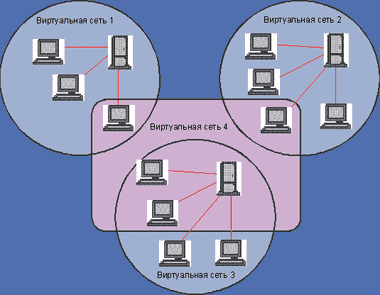
\includegraphics[scale=0.55]{pictures/vlan_net_example}
\caption{VLAN сеть}
\label{pic:vlan_net_example}
\end{figure}

Сеть любого крупного предприятия, а тем более провайдера, не может функционировать без применения VLAN, посколько объемы данных колоссальны. Применение данной технологии дает следующие преимущества:
\begin{itemize}
\item группирование устройств по функционированию;
\item уменьшение количества широковещательного трафика в сети;
\item увеличение безопасности сети;
\item увеличение управляемости сети;
\end{itemize}

Традиционно разделение сети на виртуальные сегменты выполняется по следующим критериям:
\begin{itemize}
\item по порту;
\item по mac-адресу;
\item по протоколу;
\end{itemize}

В данной работе интерес представляет разделение на сегменты по протоколу. Обычно производится по данным сетевого (IP) и транспортного уровня (TCP/UDP), что лишает провайдеров возможности использовать протоколы более высоких уровней для классификации трафика и его последующей обработки. Разрабатываемый сервис будет работать во VLAN сетях, предоставляя возможность тегирования определенного трафика (добавления метки пакету).

В данной реализации метка будет присваиваться в зависимости от того, к какому протоколу принадлежит пакет. На рисунке~\ref{pic:vlan_tag} показана структура метки согласно IEEE 802.1Q - стандарта, описывающего процедуру тегирования трафика для передачи информации о принадлежности к VLAN.
\begin{figure}
\centering
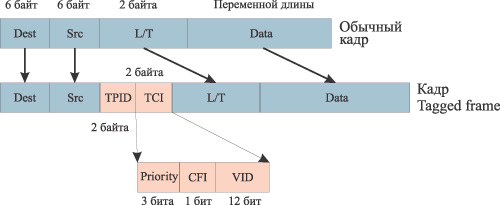
\includegraphics[scale=0.55]{pictures/vlan_tag}
\caption{VLAN метка}
\label{pic:vlan_tag}
\end{figure}

Размер тега - 4 байта. Он состоит из следующих полей:
\begin{itemize}
\item идентификатор протокола тегирования (Tag Protocol Identifier, TPID), размер поля - 16 бит, указывает какой протокол используется для тегирования, для 802.1Q используется значение 0x8100;
\item приоритет (Priority, PCP), размер поля - 3 бита, используется стандартом IEEE 802.1P для задания приоритета передаваемого трафика;
\item идентификатор канонического формата (Canonical Format Idicator, CFI), размер поля - 1 бит, указывает на формат mac-адреса, используется для совместимости между сетями Ethernet и Token Ring;
\item идентификатор VLAN (VLAN Identifier, VID), размер поля - 12 бит, указывает какому сегменту виртуальной сети принадлежит пакет, диапазон возможных значений от 0 до 4095;
\end{itemize}

Теоритический предел идентификаторов виртуальных сетей равен 4095 - на сегодняшний день этого недостаточно. Для решения этой проблемы используют технологию QinQ (стандарт IEEE 802.1AD), которая позволяет использовать внутри пакета две метки. Это расширяет количество идентификаторов до 16777216. Вторая метка имеет такую же структуру, как и первая, единственное отличие в значении поля TPID - в случае 802.1AD используется 0x88A8.


\section{Обзор существующих решений}
Системы DPI приобретают все большую популярность, несмотря на высокую стоимость. Сейчас почти у каждого большого вендора есть свое решение. У Cisco это Cisco SCE, у Huawei - SIG9800, у Juniper - VXA. Есть и менее известные компании, которые производят преимущественно оборудование DPI, например Allot или Inline Telecom.

Все эти решения являются сложными аппаратно-программными комплексами, поэтому не представляют большого интереса в рамках данной работы. Далее рассмотрены чисто программные решения, функциональные возможности  и цели которых схожи с разрабатываемым сервисом.
\subsection{Проет OpenDPI}
OpenDPI - библиотека для классификации сетевого трафика на основе технологии глубокого анализа пакетов. Она является свободной и распространяется под лицензией LGPLv3.

OpenDPI построен на базе продукта PACE, который разрабатывается компанией Ipoque, заимствовав многие особенности оттуда. Сам проект PACE является коммерческим и в рамках данной работы не рассматривается.

Основные особенности:
\begin{itemize}
\item не требует наложений патчей на ядро и iptables;
\item работает в виде модуля ядра и использует библиотеку xtables для внутренних нужд;
\item написан полностью на C, что повышает производительность;
\item для обнаружения используются модули, написанные на C, а не список регулярных выражений;
\item последняя версия библиотеки (v3.10, 2012 год) поддерживала порядка 100 протоколов;
\end{itemize}

В данный момент проект OpenDPI не поддерживается.

\subsection{Проект nDPI}
nDPI - библиотека, основанная на OpenDPI, поддерживаемая компаний ntop~\cite{ntop_company}. Это мощное DPI-решение, которое постоянно дорабатывается и улучшается и, на сегодняшний день, является самым продвинутым программным решением DPI для архитектуры x86\_64.

Основные особенности:
\begin{itemize}
\item не требует наложений патчей на ядро;
\item библиотека написана на языке C, что повышает производительность;
\item для обнаружения используются как модули на языке C, так и описание протокола в виде файла определенной структуры;
\item поддерживается более 150 протоколов, список которых постоянно пополняется;
\item работает под Linux и Windows;
\end{itemize}

Сама по себе библиотека nDPI предоставляет API для разработки конкретных сетевых приложений. Так она используется в других продуктах компании, например приложениях ntopng и nProbe. Поэтому рассматривать nDPI как прямой аналог разрабатываемого сервиса нельзя.


\section{Быстрая обработка пакетов}
Разрабатываемый сервис должен иметь высокие показатели производительности. Этого нельзя добиться просто используя более быстрый чип на сетевой карте, требуется использовать все возможности современных вычислительных систем, а также различные техники ускорения обработки.

\subsection{Возможности вычислительных систем}
\paragraph{Кэши}

На рисунке~\ref{pic:memory_schema} показаны различные уровни памяти современных CPU и примерное время доступа к ним. Такая архитектура введена для того, чтобы минимизировать время доступа программ к данным. Чем выше по иерархии находятся необходимые данные, тем выше производительность приложения в целом.
\begin{figure}[h]
\centering
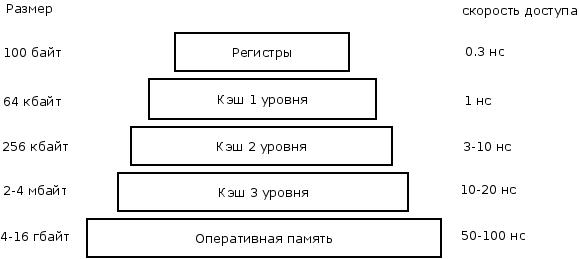
\includegraphics[scale=0.7]{pictures/memory_schema}
\caption{Иерархия памяти}
\label{pic:memory_schema}
\end{figure}

Для сокращения времени доступа к памяти данные могут быть помещены в кэш до того, как они действительно понадобятся. Такой подход реализуется как программно (software prefetching), так и на уровне железа (hardware prefetching).

\paragraph{TLB}

TLB~\cite{modern_os} представляет собой кэш ограниченного размера, хранящий отображение виртуальных адресов памяти в физические. При обращении к данным по виртуальному адресу просматриваются записи в TLB и, если нужная запись присутствует, возвращается физический адрес. В этом случае задержка несоизмеримо мала. В противном случае, когда нужной записи в кэше нет, требуется выполнять преобразование виртуального адреса в физический с последующим сохранением данных в TLB, что занимает несколько тактов процессора и негативно сказывается на производительности приложения, запросившего данные.

\paragraph{DMA}

DMA~\cite{modern_os} позволяет различным устройствам ввода-вывода обращаться к памяти напрямую, без привлечения центрального процессора. Однако, процессор должен подготовить для этого буфер в памяти и передать указатель на него устройству, которому необходим DMA, например сетевой карте. Таким образом, сетевая карта сможет считывать и записывать данные, используя этот буфер, вне зависимости от занятости процессора. Существует еще один подход под названием DCA. Он позволяет устройствам ввода-вывода записывать данные напрямую в кэш. Например, сетевая карта может помещать в кэш входящие пакеты, минуя оперативную память и не привлекая процессор.

Все это повышает скорость обработки засчет ликвидации копирования данных из памяти в процессор.

\paragraph{RSS}

Современные сетевые карты имеют несколько RX и TX очередей. Для утилизации всей пропускной способности сетевая карта может помещать пакеты в различные очереди, а каждая очередь может обрабатываться отдельным ядром процессора.

Для разделения пакетов по очередям используют подсчет хэша, соответственно трафик с одним значением хэша попадает в одну очередь, со вторым значением в другую. Такой подход позволяет масштабировать обработку данных, обрабатывая разные очереди на разных ядрах, тем самым повышая общую производительность системы.

\paragraph{Другие возможности}

Некоторые операции, такие как подсчет хэша и валидация контрольных сумм, могут быть реализованы в самих сетевых картах. Это делается для того, чтобы не нагружать процессор дополнительными вычислениями. Например, современные карты сами считают CRC для Ethernet кадров. Схожие возможности реализованы и для протоколов более высоких уровней, таких как IP и TCP/UDP.

\subsection{Техники ускорения обработки}
Фреймворки используют многочисленные техники ускорения. Некоторые их них совершенно новые в сфере обработки пакетов (не использовать стандартный сетевой стек, избегать копирования пакетов, выделять память заранее), а некоторые давно используются в современных операционных системах (режим опроса, обработка партиями).

\paragraph{Стандартный сетевой стек ядра}

Ядро выполняет большую работу по обработке трафика, анализируя пакеты, пропуская каждый из них через стек протоколов, на что тратится время. Основная задача фреймворков - как можно быстрее доставлять пакеты в режим пользователя, в котором уже реализуется обработка трафика в соответствие с логикой разрабатываемого приложения. Поэтому дополнительная обработка пакетов ядром, которая, к тому же, требует большого количества времени, не имеет смысла.

\paragraph{Копирование пакетов}

При отправке пакета, используя традиционный интерфейс системы, пакет необходимо скопировать из пользовательского сокета в буффер ядра (или наоборот). Это вносит дополнительную задержку в обработку, которых стараются избегать фреймворки, выделяя для этого буфер в памяти, который используется и приложенияем пользователя, и обработчиками пакетов. Сетевая карта считывает/записывает данные из/в область памяти (через DMA), а приложение пользователя записывает/считывает данные из этой же области.

Время копирования пакета напрямую зависит от его длины, поэтому время пересылки коллекции пакетов из сетевой карты в определенную область памяти не является постоянной величиной и меняется, в зависимости от длины каждого пакета в коллекции.

Еще одно преимущество - это возможность легко реализовывать приложения пересылки данных. Для этого не нужно копировать полученные пакеты в какой-то буфер, используемый для последующей отправки. Достаточно пометить пакет как "готовый для отправки".

\paragraph{Преждевременное выделение памяти}

Выделение памяти осуществляется в ядре операционной системы. Это может быть необходимо, когда буфер для приема пакетов не имеет достаточную длину для сохранения вновь полученного пакета. Выделение памяти приводит к системному вызову, что вносят дополнительную задержку в обработку. Аналогичная ситуация с буфером для отправки пакетов.

В фреймворках быстрой обработки пакетов память, необходимая для работы, выделяется заранее, на этапе инициализации и запуска приложения. Это позволяет избежать частых системных вызовов, повысив общую производительность. Так как размер выделенной памяти не может быть изменен в режиме реального времени, он должен быть достаточным для всех нужд приложения.

\paragraph{Режим опроса}

Раньше обработка пакетов осуществлялась через прерывания - когда на сетевой карте появлялся новый пакет, происходило прерывание и ядро обрабатывало этот пакет. При высоких скоростях трафика  ядро не успевало обрабатывать все прерывания, из-за чего страдала производительность. В современных системах при высоких нагрузках происходит переключение режима обработки с прерываний на режим опроса (polling)~\cite{modern_os}, при котором в цикле выполняется опрос сетевой карты на предмет появления новых данных.

Такой подход реализован не только в современных ОС, но и в фреймворках быстрой обработки пакетов.

\paragraph{Большие страницы}

Для того, чтобы избежать промахов в TLB, могут использоваться большие страницы памяти (huge pages)~\cite{linux_programming}. Размер страницы, обычно, увеличивается с 4 Кбайт до 2 Мбайт. Все это приводит к минимизации времени доступа к данным, находящимся в больших страницах памяти.

Детально, увеличение размера страницы приводит к сокращению числа записей в TLB, например для последних процессоров Intel с 256 записей (4 КБайт) до 32 (2 Мбайта).

\paragraph{Обработка партиями}

Практически все фреймворки предоставляют API для получения пакетов с сетевой карты.  Каждый вызов функции требует определенного количества процессорного времени, поэтому требуется, по возможности, минимизировать количество таких вызовов. Это решается предоставлением такого API, который за один вызов получает не один пакет, а партию, тем самым разделив стоимость вызова на несколько пакетов сразу.

\subsection{{PF\_RING}}
Является одним из наиболее популярных фреймворков для обработки пакетов. В данный момент поддерживается компанией ntop, состоит из набора модулей. Модуль ядра PF\_RING и драйвера распространяются под лицензией GNU GPLv2, а библиотека для пространства пользователя под лицензией LGPLv2.1 и доступна в формате исходного кода. На рисунке~\ref{pic:pfring_example} показана концептуальная схема приложения, использующего PF\_RING.
\begin{figure}[h]
\centering
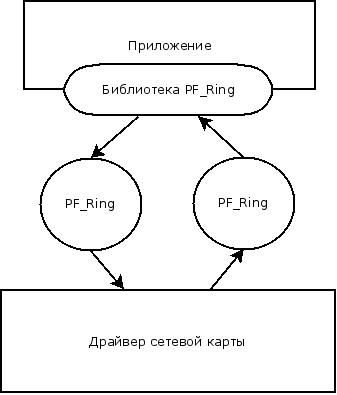
\includegraphics[scale=0.7]{pictures/pfring_example}
\caption{Использование PF\_RING}
\label{pic:pfring_example}
\end{figure}

Для получения высоких показателей производительности рекомендуется использовать улучшенную версию фреймворка - PF\_RING ZC (Zero Copy). Точная архитектура этой версии неизвестна, так как продукт является коммерческим. Согласно данным компании ntop, фреймворк основан на библиотеке libZero и его производительность - line rate на 10 Гбит/сек. Список поддерживаемых сетевых карт мал, так, например, для сетевых карт Intel доступны только драйвера e1000e, igb, ixgbe.

Основные особенности PF\_RING:
\begin{itemize}
\item использует большие страницы;
\item использует DMA;
\item использует прерывания только для выхода из заблокированного системного вызова, в остальном используется режим опроса;
\item предоставляет API для обработки партиями;
\item не использует системные вызовы для обработки пакетов;
\item не требует патчей на ядро, использует модули;
\end{itemize}

\subsection{DPDK}
Разработанный и поддерживаемый компанией Intel, фреймворк DPDK~\cite{dpdk_descr} является наиболее популярным и привлекательным для применения в разработке различных сетевых приложений. Строго говоря, DPDK - это набор программных библиотек, которые могут улучшить производительность при обработке пакетов. Является полностью свободным программным обеспечением и рапространяется под лицензией Open Source BSD.

Основная цель DPDK не просто ускорить обработку пакетов, но и предоставить набор полезных библиотек, которые позволят разработчикам создавать собственные сетевые приложения. На рисунке~\ref{pic:dpdk_eal} приведены основные библиотеки DPDK с наиболее значимой библиотекой, называемой Environment Abstraction Layer (rte\_eal).
\begin{figure}
\centering
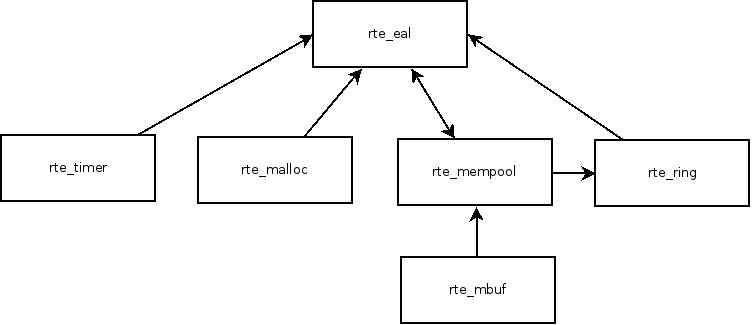
\includegraphics[scale=0.5]{pictures/dpdk_eal}
\caption{Основные библиотеки DPDK}
\label{pic:dpdk_eal}
\end{figure}

Главная библиотека rte\_eal используется для того, чтобы скрыть детали реализации на уровне железа и операционной системы от приложения пользователя и других библиотек. В этой библиотеке реализована инициализация всех ресурсов, таких как память, таймеры и компоненты шины данных. Использование библиотеки rte\_timer позволяет вызывать функции асинхронно, один раз или периодически. Точное начало отсчета времени обеспечивается через EAL. Компонент rte\_malloc используется для выделения памяти в больших страницах для использования памяти более эффективно. Библиотека rte\_mbuf предоставляет буфера для хранения пакетов, которые могут адаптироваться для хранения любых данных. Все буфера создаются при запуске приложения. rte\_ring предоставляет буфера фиксированного размера, основная особенность которых состоит в том, что они реализуют идеологию lock free, т.е. одновременно несколько потоков могут писать в буфер и читать из него. Используются для быстрого взаимодействия между различными потоками. rte\_mempool используется для сохранения объектов.

Все это лишь малая часть библиотек, поставляемых DPDK. Доступны такие библиотеки, как rte\_hash для вычесления хэша, rte\_cofig для удобного описаний и парсинга конфигураций и многие другие.

DPDK предоставляет большой список драйверов для физических и виртуальных интерфейсов. Для того, чтобы использовать эти драйвера, необходимо привязать сетевую карту к нужному драйверу. Ядро Linux не имеет доступа к устройству, пока его обслуживает драйвер DPDK. Ниже представлен неполный список доступных драйверов:
\begin{itemize}
\item xenvirt
\item vmxnet3
\item virtio
\item ixgbe
\item i40e
\item e1000
\end{itemize}

Основные особенности DPDK:
\begin{itemize}
\item использует большие страницы;
\item использует DMA;
\item не использует прерывания, только режим опроса;
\item не использует системные вызовы;
\item не требует патчей на ядро, в основном используется модуль igb\_uio;
\item большой набор поддерживаемых сетевых карт;
\item высокие показатели производительности (10 Гбит/сек на 1 ядре);
\item широкий набор дополнительных библиотек;
\item API для обработки пакетами;
\end{itemize}

\section{Постановка задачи}
Учитывая все проблемы интернет-провайдеров, описанные выше, а также проанализировав технологию DPI и доступные фреймворки быстрой обработки пакетов, необходимо реализовать сетевой сервис классификации трафика на основе технологии DPI, который должен:
\begin{itemize}
\item работать с любыми Ethernet картами;
\item автоматическое определять нужный драйвер;
\item выполнять функцию сетевого экрана;
\item выполнять функцию граничного маршрутизатора в MPLS сети;
\item выполнять тегирование трафика согласно 802.1Q и 802.1AD;
\item поддерживать конфигурирование на каждый порт;
\item использовать фреймворк DPDK и все его потенциальные возможности;
\item собирать статистику по каждому протоколу;
\end{itemize}

Разрабатываемый сервис должен быть полностью законченным приложением, а не отдельной библиотекой, предоставляющей API, а также должен быть покрыт модульными тестами. Поддерживаемые протоколы:
\begin{itemize}
\item HTTP;
\item SIP;
\item RTSP;
\item RTP;
\end{itemize}

На вход данного сервиса допускается только Ethernet/IP/TCP(UDP) трафик, который может быть тегированным. Все остальные виды трафика будут блокироваться.

\paragraph{Выводы}

В рамках данного раздела были изучены возможные варианты применения технологии DPI в сетях интернет-провайдеров. Рассмотрены случаи использования сервиса на основе DPI в качестве межсетевого экрана, граничного маршрутизатора в MPLS сетях, а так же возможность его использования для тегирования трафика. Для увеличения производительности были приведены некоторые техники ускорения, а также проанализированы фреймворки быстрой обработки пакетов. В конце раздела представлен полный список требований к разрабатываемому сервису.

\chapter{Конструкторский раздел}
\label{cha:design}
\section{Функциональная схема}
Схема системы в нотации IDEF0 представлена на рисунке~\ref{pic:idef0_schema}.
\begin{figure}
\centering
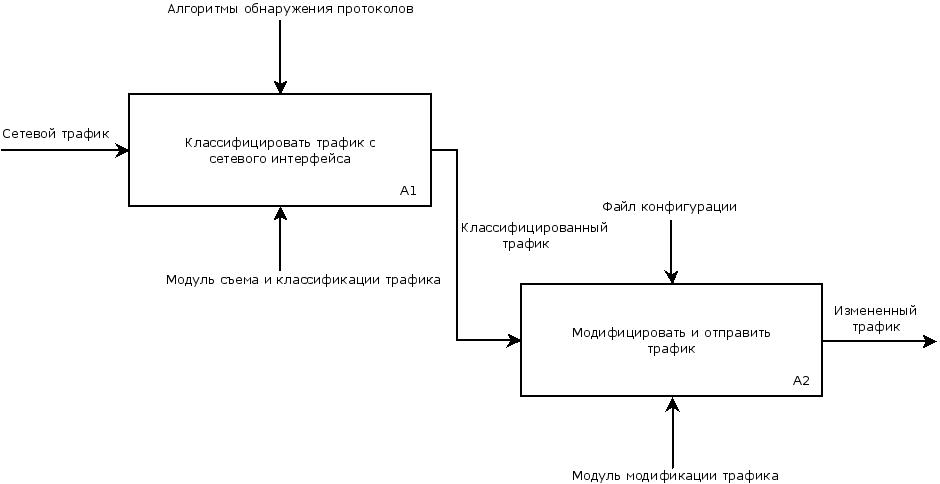
\includegraphics[scale=0.5]{pictures/idef0_schema}
\caption{Схема IDEF0}
\label{pic:idef0_schema}
\end{figure}

Система состоит из двух главных модулей:
\begin{itemize}
\item модуль съема и классификации трафика;
\item модуль модификации трафика;
\end{itemize}

Функциональные требования для модуля съема трафика:
\begin{itemize}
\item съем трафика с сетевого интерфейса;
\item определение класса трафика, используя алгоритмы обнаружения;
\item подсчет статистики по каждому классу трафика;
\end{itemize}

Функциональные требования для модуля модификации трафика:
\begin{itemize}
\item добавление MPLS метки;
\item тегирование VLAN;
\item блокировка нежелательного трафика;
\item отправка трафика в соответствующий порт;
\end{itemize}

\section{Диаграмма состояний}
На рисунке~\ref{pic:state_diagram} показана диаграмма состояний системы с момента запуска и вплоть до получения сигнала о завершении.
\begin{figure}[h]
\centering
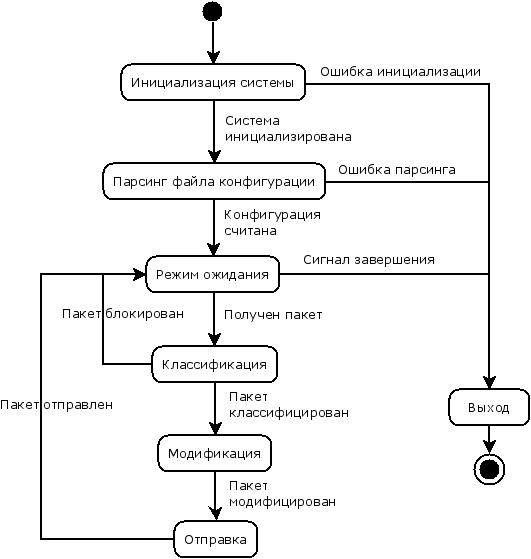
\includegraphics[scale=0.6]{pictures/state_diagram}
\caption{Диаграмма состояний}
\label{pic:state_diagram}
\end{figure}

В момент инициализации происходит выделение необходимого количества памяти под входные и выходные буфера, инициализация сетевых интерфейсов, привязка потоков к конкретным ядрам процессора. Далее выполняется считывание файла конфигурации, структура которого описана ниже. После выполнения этих операций система переходит в режим ожидания, в котором выполняется опрос сетевой карты на предмет появления новых пакетов. Каждый новый пакет проходит классификацию и, если для заданного класса трафика не предусмотрена блокировка, модификацию с последующей отправкой в нужный порт.

\section{Архитектура сервиса}
На рисунке~\ref{pic:concept_schema} представлена архитектура разрабатываемого сервиса на примере обработки трафика с двух сетевых интерфейсов.
\begin{figure}[h]
\centering
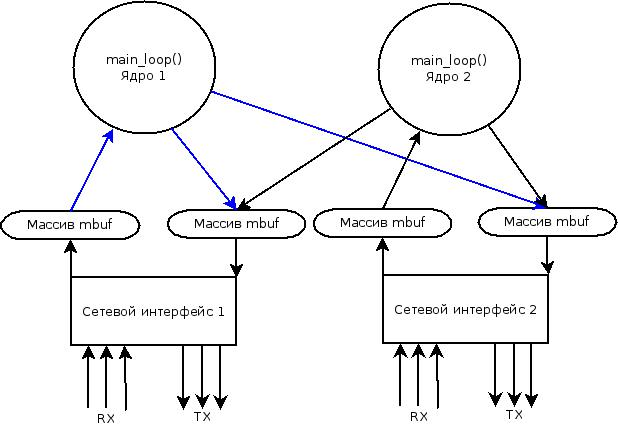
\includegraphics[scale=0.6]{pictures/concept_schema}
\caption{Архитектура сервиса}
\label{pic:concept_schema}
\end{figure}

Пакеты поступают на RX очереди сетевой карты. Количество очередей зависит от самой сетевой карты, но в данной работе используется одна RX очередь. Далее полученные пакеты сохраняются (через DMA) в массив структур mbuf, описанных в DPDK.

При запуске системы каждому сетевому интерфейсу назначается ядро, на котором запускается главный цикл обработки, таким образом одну сетевую карту обслуживает одно ядро. Случай, когда разные ядра обслуживают разные RX очереди одной сетевой карты в данной работе не рассматривается.

В главном цикле вычитываются пакеты из массива структур, производится их обработка, а затем они помещаются  в выходной массив структур mbuf нужного интерфейса. Промежуточный массив нужен для того, чтобы не вызывать часто API для отправки данных с сетевой карты, так как это снижает производительность. Вместо этого данные помещаются в буфер и с некоторой периодичностью извлекаются из него, помещаясь в TX очередь интерфейса.

\subsection{Выходные очереди}
Количество выходных очередей также зависит от самой сетевой карты, но в данной работе используется одна TX очередь на каждый сетевой интерфейс.

К входному массиву mbuf происходит обращение только из одного ядра, поэтому обеспечивать защищенность этого ресурса не требуется. С выходным массивом все иначе - несколько ядер одновременно могут обращаться к нему, поэтому требуется использовать какой-то подход, гарантирующий безопасность этого ресурса.

Наиболее распространенным является подход с использованием примитивов синхронизации, таких как мьютексы или семафоры. В данной работе не рассматривается, так как использует системные вызовы и требует больших временных затрат, что при высоких нагрузках плохо сказывается на производительности.

Еще одним подходом является разделение данных по ядрам. Именно он применен в данной работе для организации выходного массива mbuf. Для этого создается матрица, число строк которой равно числу ядер в системе, а количество столбцов - числу сетевых интерфейсов (рисуное~\ref{pic:mbuf_matrix}). Элементом такой матрицы является массив mbuf. Каждый раз, когда требуется записать/считать данные в/из выходного буфера, из матрицы извлекается элемент с индексом [номер ядра][номер порта] и дальнейшая работа производится с ним. Такой подход не требует дополнительных действий по обеспечению безопасности, т.к. каждое ядро использует собственную переменную.
\begin{figure}
\centering
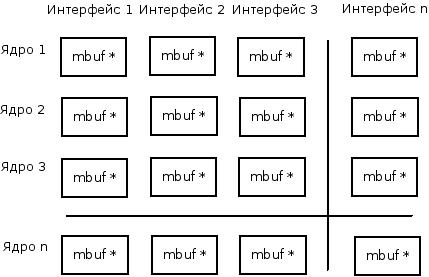
\includegraphics[scale=0.6]{pictures/mbuf_matrix}
\caption{Матрица массивов mbuf}
\label{pic:mbuf_matrix}
\end{figure}

\subsection{Статистика}
Разрабатываемый сервис должен вести статистику по общему количеству полученных и отправленных пакетов, а также статистику по каждому поддерживаемому протоколу.

Общую статистику можно получить через DPDK, используя функцию rte\_eth\_stats\_get(), которой в качестве параметров передается номер порта и структура для заполнения. Сам подсчет реализуется драйвером соответствующей карты.

Статистику по каждому протоколу необходимо реализовывать вручную. Простой способ - это хранить счетчик для каждого типа протокола и, при обнаружении соответствующего пакета, увеличивать его. Так как обновление счетчика производится с разных ядер, требуется защита переменной. Здесь, как и в случае с выходным буфером, используется массив счетчиков (рисунок~\ref{pic:counters}). Полная статистика по конкретному протоколу вычисляется как сумма счетчиков на каждом ядре.
\begin{figure}
\centering
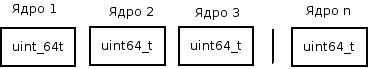
\includegraphics[scale=0.6]{pictures/counters}
\caption{Массив счетчиков}
\label{pic:counters}
\end{figure}

Подход с разделением данных по ядрам имеет скрытую угрозу производительности. Связано это с организацией памяти современных компьютеров, а именно с кэшом. Обычно, размер линейки кэша 64 байта. Допустим, мы используем счетчики размером 8 байт, то есть в одну линейку укладывается 8 таких счетчиков. Изменение хотя бы одного счетчика приводит к инвалидации и обновлению всей линейки памяти, а если такая линейка присутствует в кэше других ядер, то и к синхронизации с ними.

Вся работа по обеспечению когерентности кэшей выполняется протоколом MESI на уровне процессора. Если данные присутствуют в разных кэшах процессора, то при их модификации шлется RFO как сигнал о том, что данные больше не действительны и требуется обновить их. Многочисленные запросы RFO опасны так же, как промахи в кэш, так как сильно сказываются на производительности приложения.

Для решения этой проблемы в рамках данной работы используется стратегия выравнивания данных по размеру линейки кэша. Основная идея заключается в том, что в одну линейку помещают только одно изменяемое значение. В результате такая запись будет присутствовать в кэше только того ядра, который с ней работает, что полностью исключает возникновение RFO и повышает производительность.

\section{Поддерживаемые протоколы}
Детальное описание каждого из протоколов, поддерживаемых сервисом, выходит за рамки работы. Ниже приведены лишь их структуры и алгоритмы обнаружения.

\subsection{HTTP}
Обмен сообщениями при использовании HTTP идет по схеме "запрос-ответ". Каждое HTTP-сообщение имеет структуру, приведенную в таблице~\ref{tbl:http_structure}.
\begin{table}
\centering
\caption{Структура HTTP}
\label{tbl:http_structure}
\begin{tabular} {| c |} 
\hline
Стартовая строка\\
\hline
Заголовки\\
\hline
Пустая строка\\
\hline
Тело сообщения\\
\hline
\end{tabular}
\end{table}

Заголовки и тело сообщения могут отсутствовать, но стартовая строка является обязательной, так как указывает на тип запроса/ответа. Запрос отправляется в формате: "тип\_запроса адрес версия\_протокола". Ответ имеет формат: "версия\_протокола код\_возврата пояснения".

Список запросов, согласно~\cite{http_rfc}: OPTIONS, GET, HEAD, POST, PUT, DELETE, TRACE, CONNECT.

Пример запроса:
\begin{lstlisting}
GET HTTP://server/path/test.html HTTP/1.1
\end{lstlisting}


В рамках данной работы поддерживается только HTTP версии 1.1. Проанализировав структуру HTTP, был разработан простой протокол обнаружения, основанный только на типах запросов и версии протокола. Блок-схема приведена на рисунке~\ref{pic:http_alg}.
\begin{figure}
\centering
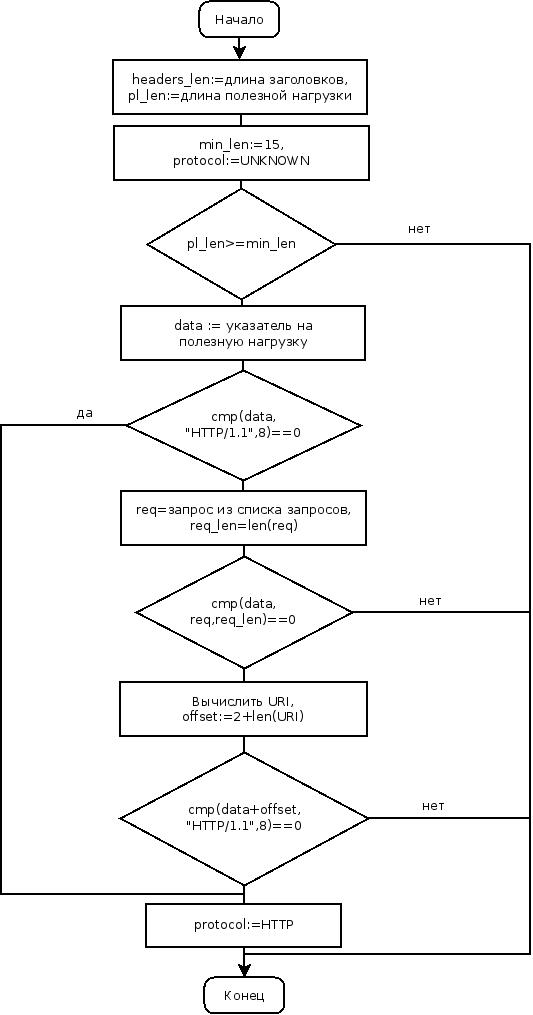
\includegraphics[scale=0.5]{pictures/http_alg}
\caption{Алгоритм обнаружения HTTP}
\label{pic:http_alg}
\end{figure}

\subsection{SIP}
Сообщения протокола SIP представляют собой последовательности текстовых строк (запросы и ответы). Структура и синтаксис идентичны используемым в протоколе HTTP.

Стартовая строка - начальная строка любого SIP-сообщения. Если сообщение является запросом, в ней указывается типа запроса, адресат и номер версии протокола. Если сообщение является ответом - указывается номер версии, тип ответа и короткая расшифровка.

Заголовки сообщений содержат информацию, необходимую для обработки сообщения.

Тело сообщения содержит описание сеансов связи. Не все запросы содержат тело (например, BYE).

Список запросов, согласно~\cite{sip_rfc}: INVITE, ACK, BYE, CANCEL, REGISTER, OPTIONS, PRACK, SUBSCRIBE, NOTIFY, PUBLISH, INFO, REFER, MESSAGE, UPDATE.

Пример запроса:
\begin{lstlisting}
INVITE sip:nikolia@example.ru SIP/2.0
\end{lstlisting}

Проанализировав структуру протокола SIP был разработан алгоритм обнаружения, блок-схема которого приведена на рисунке~\ref{pic:sip_alg}.
\begin{figure}
\centering
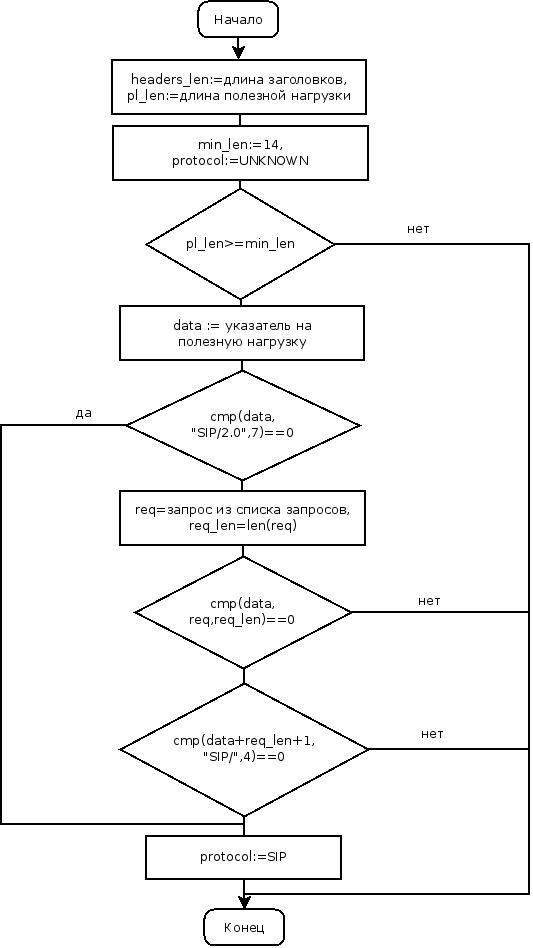
\includegraphics[scale=0.6]{pictures/sip_alg}
\caption{Алгоритм обнаружения SIP}
\label{pic:sip_alg}
\end{figure}

\subsection{RTSP}
По синтаксису и операциям протокол RTSP похож на HTTP, хотя есть и ряд отличий, например в случае RTSP и сервер и клиент могут генерировать запросы.

Запрос на сервер посылается в текстовом виде в формате: "тип\_запроса абсолютный\_адрес контент версия\_протокола". Вместе с запросом могут быть переданы дополнительные служебные поля (на новых строчках запроса). Ответ посылается также в текстовом виде и содержит номер версии, тип ответа и короткую расшифровку.

Список запросов, согласно~\cite{rtsp_rfc}: DESCRIBE, OPTIONS, PLAY, PAUSE, RECORD, REDIRECT, SETUP, ANNOUNCE, GET\_PARAMETER, SET\_PARAMETER, TEARDOWN.

Пример запроса:
\begin{lstlisting}
PLAY RTSP://server/path/test.mpg RTSP/1.0
\end{lstlisting}

Проанализировав структуру протокола RTSP, был разработан алгоритм обнаружения, блок-схема которого приведена на рисунке~\ref{pic:rtsp_alg}.
\begin{figure}
\centering
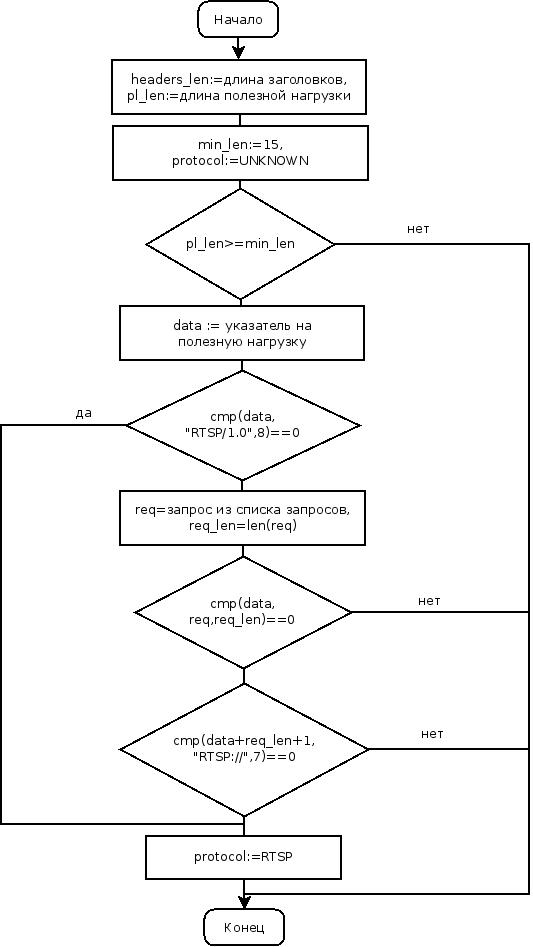
\includegraphics[scale=0.6]{pictures/rtsp_alg}
\caption{Алгоритм обнаружения RTSP}
\label{pic:rtsp_alg}
\end{figure}

\subsection{RTP}
Структура пакета RTP, согласно~\cite{rtp_rfc}, приведена в таблице~\ref{tbl:rtp_structure}.
\begin{table}
\centering
\caption{Структура RTP}
\label{tbl:rtp_structure}
\begin{tabular} {| c | c | c | c | c | c | c | c |} 
\hline
+Биты & 0-1 & 2 & 3 & 4-7 & 8 & 9-15 & 16-31\\
\hline
0 & Ver. & P & X & CC & M & PT & Порядковый номер\\
\hline
32 & \multicolumn{7}{ c |}{Метка времени}\\
\hline
64 & \multicolumn{7}{ c |}{SSRC-идентификатор}\\
\hline
96, если & \multicolumn{7}{ c |}{[CSRC-идентификаторы]}\\
CC>0 & \multicolumn{7}{ c |}{}\\
\hline
96+(CCx32), & \multicolumn{6}{ c |}{[Заголовок расширения -} & [Заголовок расширения - количество\\
если X=1 & \multicolumn{6}{ c |}{определенное профилем значение]} & блоков данных по 32 бита(EHL)]\\
\hline
96+ & \multicolumn{7}{ c |}{[Заголовок расширения - блоки данных]}\\
(CCx32)+32 & \multicolumn{7}{ c |}{}\\
\hline
96+(CCx32) & \multicolumn{7}{ c |}{}\\
+X* & \multicolumn{7}{ c |}{Данные}\\
(32+32xEHL) & \multicolumn{7}{ c|}{}\\
\hline
если P=1 & \multicolumn{6}{ c |}{Выравнивание} & L\\
\hline
\end{tabular}
\end{table}

Ver (2 бита) указывает версию протокола, текущая версия 2.

P (1 бит) используется в случаях, когда RTP-пакет дополняется пустыми байтами на конце.

X (1 бит) используется для указания расширений протокола, задействованных в пакете.

CC (4 бита) содержит количество CSRC-идентификаторов, следующих за постоянным заголовком.

M (1 бит) используется на уровне приложения и определяется профилем, если поле установлено, то данные пакета имеют какое-то особое значение для приложения.

PT (7 бит) указывает формат полезной нагрузки и определяет ее интерпретацию приложением, допустимые значения: 0-34, 96-127.

SSRC (64-95 бита) указывает источник синхронизации, не может быт равным 0.

EHL (Extension Header Length) - количество 32-битных слов в блоке данных расширения заголовка.

L - последний байт в пакете, определяющий длину области заполнения в байтах (используется для выравнивания в последнем пакете).

Проанализировав структуру протокола RTP, был разработан алгоритм обнаружения, блок-схема которого приведена на рисунке~\ref{pic:rtp_alg}.
\begin{figure}
\centering
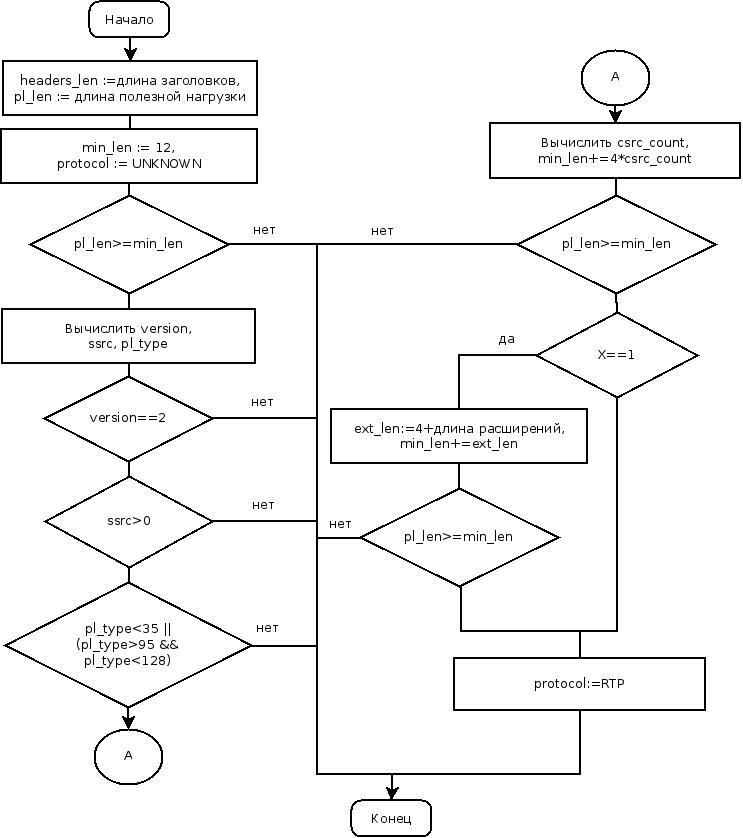
\includegraphics[scale=0.6]{pictures/rtp_alg}
\caption{Алгоритм обнаружения RTP}
\label{pic:rtp_alg}
\end{figure}


\section{Конфигурационный файл}
\subsection{Структура}
Конфигурационный файл используется для того, чтобы определить поведение сервиса при обнаружении поддерживаемых протоколов. В нем описываются порты, протоколы, которые необходимо детектировать на этом порте и набор действий, выполняемый при обнаружении.

Сам файл задается в текстовом виде и имеет следующую структуру:
\begin{center}
номер\_порта,протокол : список действий;
\end{center}

Основные особенности:
\begin{itemize}
\item между составными частями допускается любое количество пробелов;
\item список действий не может быть пустым;
\item протокол должен быть одним из списка поддерживаемых сервисом;
\item пакеты неописанных протоколов по умолчанию блокируются;
\item номер порта указывается в численном виде;
\item протокол задается большими английскими буквами;
\item UNKNOWN используется для неподдерживаемых протоколов;
\end{itemize}

\subsection{Действия и допустимые значения}
Все параметры действий указываются в круглых скобках и задаются в десятичной системе счисления. Описание действия всегда оканчивается символом ";". Порядок объявления в списке действий зависит от самого действия и описан ниже.

\paragraph{DROP}

Не имеет параметров, используется для явной блокировки определенного типа трафика. В списке действий должно располагаться первым, остальные действия, если присутствуют, не выполняются.

Пример описания:
\begin{lstlisting}
1,SIP : DROP;
\end{lstlisting}

\paragraph{OUTPUT}

В качестве параметра указывается номер выходного порта. Может использоваться несколько раз, например для реализации широковещательной рассылки. В списке действий должно быть последним действием.

Пример описания:
\begin{lstlisting}
1,SIP : OUTPUT(2);
\end{lstlisting}

\paragraph{PUSH-VLAN}

В качестве параметров указывается набор из 4 чисел, разделенных запятой, состоящий из:
\begin{itemize}
\item TPID - 0x8100 для тегирования 802.1Q и 0x88A8 для 802.1AD;
\item PCP - ограничен размером поля (3 бита);
\item CFI - ограничен размером поля (1 бит);
\item VID - ограничен размером поля (12 бит), а также зарезервированными значениями;
\end{itemize}

Может использоваться несколько раз, например для реализации QinQ. В списке действий должно располагаться до действия OUTPUT.

Пример описания:
\begin{lstlisting}
1,SIP : PUSH-VLAN(33024, 3, 1, 100);
\end{lstlisting}

\paragraph{PUSH-MPLS}

В качестве параметров указывается набор из 4 чисел, разделенных запятой, состоящий из:
\begin{itemize}
\item LABEL - ограничен размером поля (20 бит);
\item CoS - ограничен размером поля (3 бита);
\item S - ограничен размером поля (1 бит);
\item TTL - ограничен размером поля (8 бит);
\end{itemize}

Может использоваться несколько раз, например для создания стека MPLS меток. В списке действий должно располагаться до действия OUTPUT.

Пример использования:
\begin{lstlisting}
1,SIP : PUSH-MPLS(100, 3, 1, 64);
\end{lstlisting}

\chapter{Технологический раздел}
\label{cha:impl}


\section{Выбор операционной системы}
Выбор стоял только между дистрибутивами Linux, так как ключевой компонент разработки - фреймворк DPDK - не работает под управлением ОС семейства Windows. Критерии выбора:
\begin{itemize}
\item бесплатное распространение;
\item наличие менеджера пакетов, позволяющего устанавливать необходимое ПО из репозиториев;
\item простота настройки и конфигурирования необходимых компонент;
\end{itemize}

В качестве ОС для разработки и развертывания была выбрана ОС Ubuntu 14.04 Trusty, версия ядра 3.16.0-53-generic, так как она удовлетворяет всем критериям.


\section{Выбор языка программирования}
В качестве языка программирования для разработки был выбран C++, версия стандарта 11. Причины решения в пользу этого языка:
\begin{itemize}
\item DPDK написан на языке C;
\item является компилируемым, а не интерпретируемым языком;
\item высокие показатели производительности;
\item полная поддержка парадигмы ООП;
\item простота работы на низком уровне (битовые операции, потоки);
\item наличие бесплатных компиляторов, сред разработки;
\item наличие бесплатных фреймворков логирования и тестирования;
\item наличие бесплатных утилит отладки и профилирования;
\end{itemize}

Дополнительный плюс использования C++ - это широкие возможности стандартной библиотеки, например: контейнеры, алгоритмы, средства синхронизации. Все это пришлось бы реализовывать вручную при использовании языка C в качестве языка разработки.


\section{Другие инструменты}
\paragraph{Git}

В качестве системы управления версиями использовался git - на сегодняшний день является самым популярным и имеет самый широкий список функциональных возможностей.

В Ubuntu git можно установить из репозиториев следующей командой:
\begin{lstlisting}
sudo apt-get install git
\end{lstlisting}

В качестве удаленного хранилища был выбран github.com.

\paragraph{Vim}

Для C++ существует большое количество сред разработки, как платных, так и нет, например: QtCreator, Eclipse, Netbeans. Это сложные IDE с графическим интерфейсом, возможностью привязки системы контроля версий, встроенным отладчикам и т.д.

В качестве среды разработки данного сервиса был выбран текстовый редактор vim засчет его простоты, а также наличия в любом дистрибутиве Linux.

В Ubuntu vim можно установить из репозиториев следующей командой:
\begin{lstlisting}
sudo apt-get install vim
\end{lstlisting}

\paragraph{Latex}

В качестве инструмента разработки РПЗ использовалась система компьютерной верстки Latex. Выбор в пользу этой системы был сделан по следующим причинам:
\begin{itemize}
\item бесплатное распространение;
\item возможность верстки в любом текстовом редакторе (использовался vim);
\item развитые функциональные возможности (автоматическое оглавление, таблицы, формулы);
\item возможность хранить документ как набор отдельных .tex файлов;
\end{itemize}

В Ubuntu Latex можно установить из репозиториев следующей командой:
\begin{lstlisting}
sudo apt-get install texlive-full
\end{lstlisting}

\paragraph{Valgrind}

Для профилирования использования памяти, выходов за границы массивов и отдельных участков кода использовался valgrind. Выбор был сделан в пользу этого инструмента по следующим причинам:
\begin{itemize}
\item бесплатное распространение;
\item развитые функциональные возможности (построение временных графиков, отслеживание выходов за границы, области неинициализированных данных);
\item отслеживание утечек памяти (бесплатных аналогов нет);
\end{itemize}

В Ubuntu valgrind можно установить из репозиториев следующей командой:
\begin{lstlisting}
sudo apt-get install valgrind
\end{lstlisting}


\section{Структура приложения}
Первое действие, которое выполняется при запуске - это инициализация компонент DPDK. Ее должно выполнять любое приложение, использующее DPDK. Функция инициализации имеет следующую сигнатуру:
\begin{lstlisting}
int rte_eal_init(int argc, char *argv[]);
\end{lstlisting}

Процесс инициализации состоит из следующих частей:
\begin{itemize}
\item считывание данных с шины PCI с целью определения нужного драйвера сетевых устройств, их последующая инициализация;
\item создание нужного числа потоков, в зависимости от количества доступных ядер (используется pthread\_create);
\item привязка каждого потока к своему ядру (используется pthread\_setaffinity\_np);
\item выделение необходимого количества памяти в больших страницах (используется mmap);
\item инициализация внутренних структур и таймеров;
\end{itemize}

Далее выполняется инициализация системы логирования, для этого используется библиотека glog от компании Google. Функция инициализации имеет следующую сигнатуру:
\begin{lstlisting}
google::InitGoogleLogging(argv[0]);
\end{lstlisting}

Glog является бесплатной и может быть установлена из репозиториев Ubuntu следующей командой:
\begin{lstlisting}
sudo apt-get install libgoogle-glog-dev
\end{lstlisting}

После инициализации DPDK и системы логирования выполняется инициализация всех классов, использующихся в работе сервиса. Ниже подробно описан каждый из них.

\subsection{Класс Config}
Класс Config реализует все действия по работе с файлом конфигурации, ниже приведена его структура:
\begin{lstlisting}
class Config {
 public:
  explicit Config(const std::string &);
  ~Config();

  Config(const Config &) = delete;
  Config &operator=(const Config &) = delete;
  Config(Config &&) = delete;
  Config &operator=(Config &&) = delete;

  bool Initialize();
  void GetActions(const uint16_t, Actions *&);

 protected:
  bool ParsePortAndProtocol(uint16_t &, std::string &);
  bool ParseActions(Actions &, std::string &);
  bool ParseVlanData(uint16_t &, uint8_t &, uint8_t &, uint16_t &, std::string &);
  bool ParseMplsData(uint32_t &, uint8_t &, uint8_t &, uint8_t &, std::string &);

 private:
  std::string config_name_;
  std::unordered_map<uint16_t, Actions> rules_;
};
\end{lstlisting}

Конструктор принимает один параметр - имя файла конфигурации, которое сохраняется в член класса config\_name\_.

Метод Initialize() выполняет парсинг файла и сохраняет правила в член класса rules\_, который представлен в виде unordered\_map стандартной библиотеки C++. Этот вид контейнера выбран для быстрого поиска правил (O(1)). Ключ - 16 битное значение: первые 8 бит - номер порта, вторые 8 бит - протокол. Значением является набор действий, которые требуется применить к определенному типу трафика на определенном порту. Действия хранятся в контейнере vector стандартной библиотеки и описаны в конструкторском разделе.

Метод GetActions(...) выполняет поиск нужного правила в rules\_ по ключу, переданному первым параметром и, если поиск завершается удачно, сохраняет результат в переменную, переданную вторым параметром. В противном случае сохранется nullptr как индикатор того, что нужное правило не найдено. В этом случае трафик должен быть блокирован.

Исходный код этого класса находится в файлах config.h и config.cpp в папке src.

\subsection{Классы PortBase и PortEthernet}
Класс PortBase является абстрактным классом и используется в качестве базового для класса PortEthernet, ниже приведена его структура:
\begin{lstlisting}
class PortBase {
 public:
  explicit PortBase(const uint8_t);
  virtual ~PortBase() = default;

  PortBase(const PortBase &) = delete;
  PortBase &operator=(const PortBase &) = delete;
  PortBase(PortBase &&) = delete;
  PortBase &operator=(PortBase &&) = delete;

  virtual void SendOnePacket(rte_mbuf *, PortQueue *) = 0;
  virtual void SendAllPackets(PortQueue *) = 0;
  virtual void ReceivePackets(PortQueue *) = 0;
  uint8_t GetPortId() const;

 private:
  uint8_t port_id_;
};
\end{lstlisting}

Конструктор принимает один параметр - номер порта, который сохраняется в член класса port\_id\_.

Абстрактные виртуальные методы SendOnePacket(...), SendAllPackets(...) и ReceivePackets(...) реализуют логику отправки и приема пакетов на сетевом интерфейсе. Должны быть переопределены производными классами в соответствие с логикой их работы.

Так класс PortEthernet переопределяет эти методы для работы с Ethernet портами. Ниже приведены сигнатуры функций, которые используются для отправки и приема непосредственно на самом сетевом устройстве:
\begin{lstlisting}
uint16_t rte_eth_tx_burst(uint8_t port_id, uint16_t queue_id, rte_mbuf **tx_pkts, uint16_t nb_pkts);
uint16_t rte_eth_rx_burst(uint8_t port_id, uint16_t queue_id, rte_mbuf **rx_pkts, uint16_t nb_pkts);
\end{lstlisting}

Исходный код обоих классов находится в файлах port.h и port.cpp в папке src.

\subsection{Класс PortManager}
Класс PortManager отвечает за инициализацию сетевых интерфейсов, маппинг ядер и портов, инициализацию экземпляров PortEthernet. Ниже приведена его структура:
\begin{lstlisting}

class PortManager {
 public:
  PortManager();
  ~PortManager();

  PortManager(const PortManager &) = delete;
  PortManager &operator=(const PortManager &) = delete;
  PortManager(PortManager &&) = delete;
  PortManager &operator=(PortManager &&) = delete;

  bool Initialize();
  PortBase *GetPortByCore(const unsigned) const;
  PortBase *GetPortByIndex(const uint8_t) const;
  PortQueue *GetPortTxQueue(const unsigned, const uint8_t);
  unsigned GetStatsLcoreId() const;
  rte_mbuf *CopyMbuf(rte_mbuf *) const;

 protected:
  bool InitializePort(const uint8_t, const unsigned) const;
  void CheckPortsLinkStatus(const uint8_t) const;

 private:
  std::unordered_map<unsigned, rte_mempool *> mempools_; // socket->mempool
  std::unordered_map<unsigned, PortBase *> ports_map_;   // lcore->port
  std::vector<PortBase *> ports_;                        // ports
  PortQueue port_tx_table_[RTE_MAX_LCORE][RTE_MAX_ETHPORTS];
  unsigned stats_lcore_id_;
};
\end{lstlisting}

Метод Initialize() является ключевым и выполняет следующие действия:
\begin{itemize}
\item находит каждому порту свободное ядро, на котором этот порт будет обрабатываться, сохраняет полученное отображения в член класса ports\_map\_, который реализован в виде unordered\_map. Ключ - 4 байта, является идентификатором ядра, значение - экземпляр класса PortEthernet.
\item для каждого процессора создает rte\_mempool и сохраняет это отображение в mempools\_, реализованный в виде unordered\_map. Ключ - 4 байта, является идентификатором процессора, значение - rte\_mempool. Для создания пула памяти используется функция:
\begin{lstlisting}
rte_mempool *rte_pktmbuf_pool_create(const char *name, unsigned n, unsigned cache_size, uint16_t priv_size, uint16_t data_room_size, int socket_id);
\end{lstlisting}
\item инициализирует все сетевые порты, что подразумевает инициализацию входной и выходной очередей, запуск сетевого интерфейса, перевод его в неразборчивый режим (promiscuous mode), проверку состояния (link up/down). Для этого используется следующий набор функций:
\begin{lstlisting}
int rte_eth_dev_configure(uint8_t port_id, uint16_t nb_rx_queue, uint16_t nb_tx_queue, rte_eth_conf *eth_conf);
int rte_eth_rx_queue_setup(uint8_t port_id, uint16_t rx_queue_id, uint16_t nb_rx_desc, unsigned int socket_id, const rte_eth_rxconf *rx_conf, rte_mempool *mp);
int rte_eth_tx_queue_setup(uint8_t port_id, uint16_t tx_queue_id, uint16_t nb_tx_desc, unsigned int socket_id, const rte_eth_rxconf *tx_conf);
int rte_eth_dev_start(uint8_t port_id);
void rte_eth_link_get_nowait(uint8_t port_id, rte_eth_link *link);
\end{lstlisting}
\end{itemize}

Методы GetPortByCore(...) и GetPortByIndex(...) возвращают указатель на экземпляр PortEthernet по идентификатору ядра или номеру порта соответственно.

Член класса port\_tx\_table\_ используется для реализации выходного буфера, описанного в конструкторском разделе, а stats\_lcore\_id\_ - для хранения идентификатора ядра, на котором производится печать статистики.

Исходный код класса PortManager находится в файлах port\_manager.h и port\_manager.cpp в папке src. Там же определены значения некоторых переменных, требуемых для инициализации сетевых интерфейсов и пулов памяти.

\subsection{Класс PacketAnalyzer}
Класс PacketAnalyzer реализует логику DPI, его структура приведена ниже:
\begin{lstlisting}
class PacketAnalyzer {
 using SearchMethod = std::function<protocol_type(rte_mbuf *)>;

 public:
  PacketAnalyzer();
  ~PacketAnalyzer() = default;

  PacketAnalyzer(const PacketAnalyzer &) = delete;
  PacketAnalyzer &operator=(const PacketAnalyzer &) = delete;
  PacketAnalyzer(PacketAnalyzer &&) = delete;
  PacketAnalyzer &operator=(PacketAnalyzer &&) = delete;

  static PacketAnalyzer &Instance();
  protocol_type Analyze(rte_mbuf *) const;

 private:
  std::vector<SearchMethod> methods_;
};
\end{lstlisting}

Единственным членом класса является methods\_ - vector, состоящий из методов поиска. Каждый метод - это отдельный модуль на C++, реализующий детектирование конкретного протокола. Все модули располагаются в папке src/protocols и используются в PacketAnalyzer.

Метод Analyze(...) обрабатывает пакет каждым методом поиска из methods\_. В результате возвращается тип протокола или UNKNOWN, если не удалось отнести пакет ни к одному протоколу.

Исходный код класса PacketAnalyzer находится в файлах packet\_analyzer.h и packet\_analyzer.cpp в папке src.

\subsection{Класс PacketManager}
Класс PacketManager выполняет считывание пакетов с сетевой карты и их последующую обработку. Экземпляры классов Config и PortManager являются членами класса и используются им в процессе обработки трафика. Экземпляр PacketAnalyzer, хоть и не является членом класса PacketManager, используется для определения типа трафика. Ниже приведена структура этого класса:
\begin{lstlisting}
class PacketManager {
 public:
  PacketManager(const std::string &, const uint16_t);
  ~PacketManager() = default;

  PacketManager(const PacketManager &) = delete;
  PacketManager &operator=(const PacketManager &) = delete;
  PacketManager(PacketManager &&) = delete;
  PacketManager &operator=(PacketManager &&) = delete;

  bool Initialize();
  void RunProcessing();

 protected:
  void ProcessPackets(PortQueue *, const uint8_t);
  void ExecuteOutput(rte_mbuf *, const uint8_t);

  void PrintStats() const;

 private:
  Config config_;
  PortManager port_manager_;
  uint16_t stats_interval_;
};
\end{lstlisting}

Метод Initialize() вызывает одноименный метод у членов класса config\_ и port\_manager\_.

Метод RunProcessing() - это основной цикл обработки, именно этот метод  запускается на каждом ядре и в нем происходит вся логика работы сервиса. В зависимости от того, на каком ядре он запущен, выполняется считывание пакетов из нужного порта. Далее они обрабатываются методом ProcessPackets(...), в котором анализируются и, в зависимости от протокола, над ними выполняются действия, определенные в config\_. Также в рамках метода RunProcessing() выполняется отправка пакетов по истечению определенного интервала времени, проверка состояния порта (link up/down), подсчет и печать статистики.

Запуск основного цикла обработки выполняется после инициализации всех компонент и реализуется функцией:
\begin{lstlisting}
int rte_eal_mp_remote_launch(lcore_function_t *f, void *arg, rte_rmt_call_master_t call_master);
\end{lstlisting}

Исходный код класса PacketManager находится в файлах packet\_manager.h и packet\_manager.cpp в папке src. Запуск метода RunProcessing() производится из файла main.cpp в той же папке.

\section{Развертывание и запуск}
Для сборки и функционирования сервиса требуется установить дополнительные пакеты, сделать это можно следующей командой:
\begin{lstlisting}
sudo apt-get install g++ cmake libpcap-dev libfuse-dev
\end{lstlisting}

Далее требуется установить DPDK и настроить возможность использования больших страниц. Для этого нужно скачать архив с официального сайта~\cite{dpdk_descr} и выполнить следующие команды:
\begin{lstlisting}
sudo tar xf dpdk.tar.gz /opt/ && cd /opt/dpdk
make config T=x86_64-native-linuxapp-gcc
sed -ri 's,(PMD_PCAP=).*,\1y,' build/.config
sudo make

sudo mkdir p /mnt/huge
sudo mount -t hugetlbfs nodev /mnt/huge
sudo echo 64 > /sys/devices/system/node/node0/hugepages/hugepages-2048kB/nr_hugepages
\end{lstlisting}

На этом установка необходимых компонентов окончена и можно собрать проект, используя Cmake, следующими командами:
\begin{lstlisting}
mkdir build && cd build
cmake .. -DCMAKE_BUILD_TYPE=Release
make
\end{lstlisting}

\subsection{Аргументы командной строки}
Запуск сервиса производится из командной строки следующей командой:
\begin{lstlisting}
sudo ./dpdk_dpi -c <num_cores> -n1 -- --config <config_name> --stats-interval <seconds>
\end{lstlisting}
Ниже объясняется значение аргументов:
\begin{itemize}
\item -c <num\_cores> - используется DPDK для указания количества используемых ядер, задается в шестнадцатеричной системе счисления, обязательный;
\item --config <config\_name> - имя файла конфигурации, обязательный;
\item --stats-interval <seconds> - выводить статистику каждые seconds секунд, необязательный;
\end{itemize}

\subsection{Статистика}
Статистика собирается во время работы по каждому поддерживаемому протоколу и по общему числу полученных/отправленных пакетов. Подсчет ведется для каждого сетевого интерфейса.

Если при запуске задан ключ --stats-interval, то данные выводятся в стандартный поток вывода в следующем виде:
\begin{lstlisting}
=====Statistcics=====
port_id=0
 - Pkts in: 1
 - Pkts out: 0
     HTTP: 0
     SIP: 0
     RTP: 0
     RTSP: 0
port_id=1
 - Pkts in: 0
 - Pkts out: 0
     HTTP: 0
     SIP: 0
     RTP: 0
     RTSP: 0
====================
\end{lstlisting}


\section{Тестирование}
Процесс тестирования является неотъемлимой частью разработки любого программного обеспечения. Благодаря ему удается выявить ошибки как на уровне исходного кода, так и в функционировании всей системы.

В рамках разработки сервиса классификации трафика проводились следующие виды тестирования:
\begin{itemize}
\item Модульное;
\item Функциональное;
\item Нагрузочное;
\end{itemize}

\subsection{Модульное тестирование}
Целью модульного тестирования является изолирование отдельных частей программы и демонстрация того, что все отдельные части являются работоспособными. Обычно реализуется в виде тестирования отдельных участков кода, например методов класса, с использованием специализированного фреймворка.

В качестве фреймворка был выбран Gtest от компании Google. Он является бесплатным и может быть установлен из репозиториев Ubuntu следующей командой:
\begin{lstlisting}
sudo apt-get install libgtest-dev
cd /usr/src/gtest
sudo cmake CMakeLists.txt
sudo make
sudo cp *.a /usr/lib
\end{lstlisting}

В рамках модульного тестирования проверялись на корректность обнаружения протоколов все методы поиска. Также проводилось тестирование корректности использования аргументов командной строки.

Все тесты находятся в папке test и test/protocols. Ниже приведен фрагемнт кода для тестирования метода поиска протокола RTP:
\begin{lstlisting}
  TEST(RTP, BadExt) {
    uint8_t data[] = {
      0x00, 0x00, 0x00, 0x00, 0x00, 0x00,
      0x00, 0x00, 0x00, 0x00, 0x00, 0x00,
      0x08, 0x00,
  
      0x05, 0x00,
      0x00, 0x00,
      0x00, 0x00,
      0x00, 0x00,
      0x40, 0x11, // (ttl, proto)
      0x00, 0x00,
      0x00, 0x00, 0x00, 0x00,
      0x00, 0x00, 0x00, 0x00,
  
      0x00, 0x00,
      0x00, 0x00,
      0x00, 0x00,
      0x00, 0x00,
  
      0x90, 0x08, 0x00, 0x03,
      0x00, 0x00, 0x00, 0x00, // timestamp
      0x00, 0x00, 0x00, 0x01,
      0x00, 0x00, 0x00, 0x02,
      // ext data (second is absent)
      0x00, 0x00, 0x00, 0x00,
    };
    auto m = InitPacket(data, sizeof(data));
    ASSERT_EQ(PreparePacket(m), true);
    ASSERT_EQ(SearchRtp(m), UNKNOWN);
    rte_pktmbuf_free(m);
  }

  TEST(RTP, GoodWithoutCsrcAndWithoutExt) {
    uint8_t data[] = {
      0x00, 0x00, 0x00, 0x00, 0x00, 0x00,
      0x00, 0x00, 0x00, 0x00, 0x00, 0x00,
      0x08, 0x00,
  
      0x05, 0x00,
      0x00, 0x00,
      0x00, 0x00,
      0x00, 0x00,
      0x40, 0x11, // (ttl, proto)
      0x00, 0x00,
      0x00, 0x00, 0x00, 0x00,
      0x00, 0x00, 0x00, 0x00,
  
      0x00, 0x00,
      0x00, 0x00,
      0x00, 0x00,
      0x00, 0x00,
  
      0x80, 0x08, 0x00, 0x03,
      0x00, 0x00, 0x00, 0x00, // timestamp
      0x00, 0x00, 0x00, 0x01,
    };
    auto m = InitPacket(data, sizeof(data));
    ASSERT_EQ(PreparePacket(m), true);
    ASSERT_EQ(SearchRtp(m), RTP);
    rte_pktmbuf_free(m);
  }
\end{lstlisting}

Данный фрагмент содержит два модульных теста:
\begin{itemize}
\item в первом определяется RTP-пакет, в котором не хватает одного дополнительного заголовка, из-за чего метод поиска SearchRtp(...) возвращает UNKNOWN;
\item во втором определяется корректный RTP-пакет, поэтому SearchRtp(...) возвращает RTP;
\end{itemize}

Ниже приведены результаты запуска всех модульных тестов:
\begin{lstlisting}
[----------] Global test environment tear-down
[==========] 49 tests from 8 test cases ran. (4 ms total)
[  PASSED  ] 49 tests.
\end{lstlisting}

\subsection{Функциональное тестирование}
Целью функционального тестирования является проверка работоспособности всей системы в целом, а также корректности взаимодействия ее частей между собой.

В рамках функционального тестирования проверялась правильность определения типа трафика и выполнения действий над ним. Для этого использовались .pcap файлы, утилита tcpreplay для их "проигрывания" и утилита tcpdump для записи трафика с выходного интерфейса. Просмотр записанного на выходе файла осуществлялся с использованием Wireshark.

Все .pcap файлы для тестирования находятся в папке pcap. Wireshark можно бесплатно загрузить с официального сайта и установить на компьютере. Tcpdump уже установлен в Ubuntu 14.04, а tcpreplay устанавливается следующей командой:
\begin{lstlisting}
sudo apt-get install tcpreplay
\end{lstlisting}

На рисунке~\ref{pic:wireshark} показано содержимое файла, записанного на выходе, когда на входе используется файл HTTP.pcap и файл конфигурации с единственным правилом:
\begin{center}
1,HTT : PUSH-VLAN(33024,2,0,100);OUTPUT(2);
\end{center}

\begin{figure}
\centering
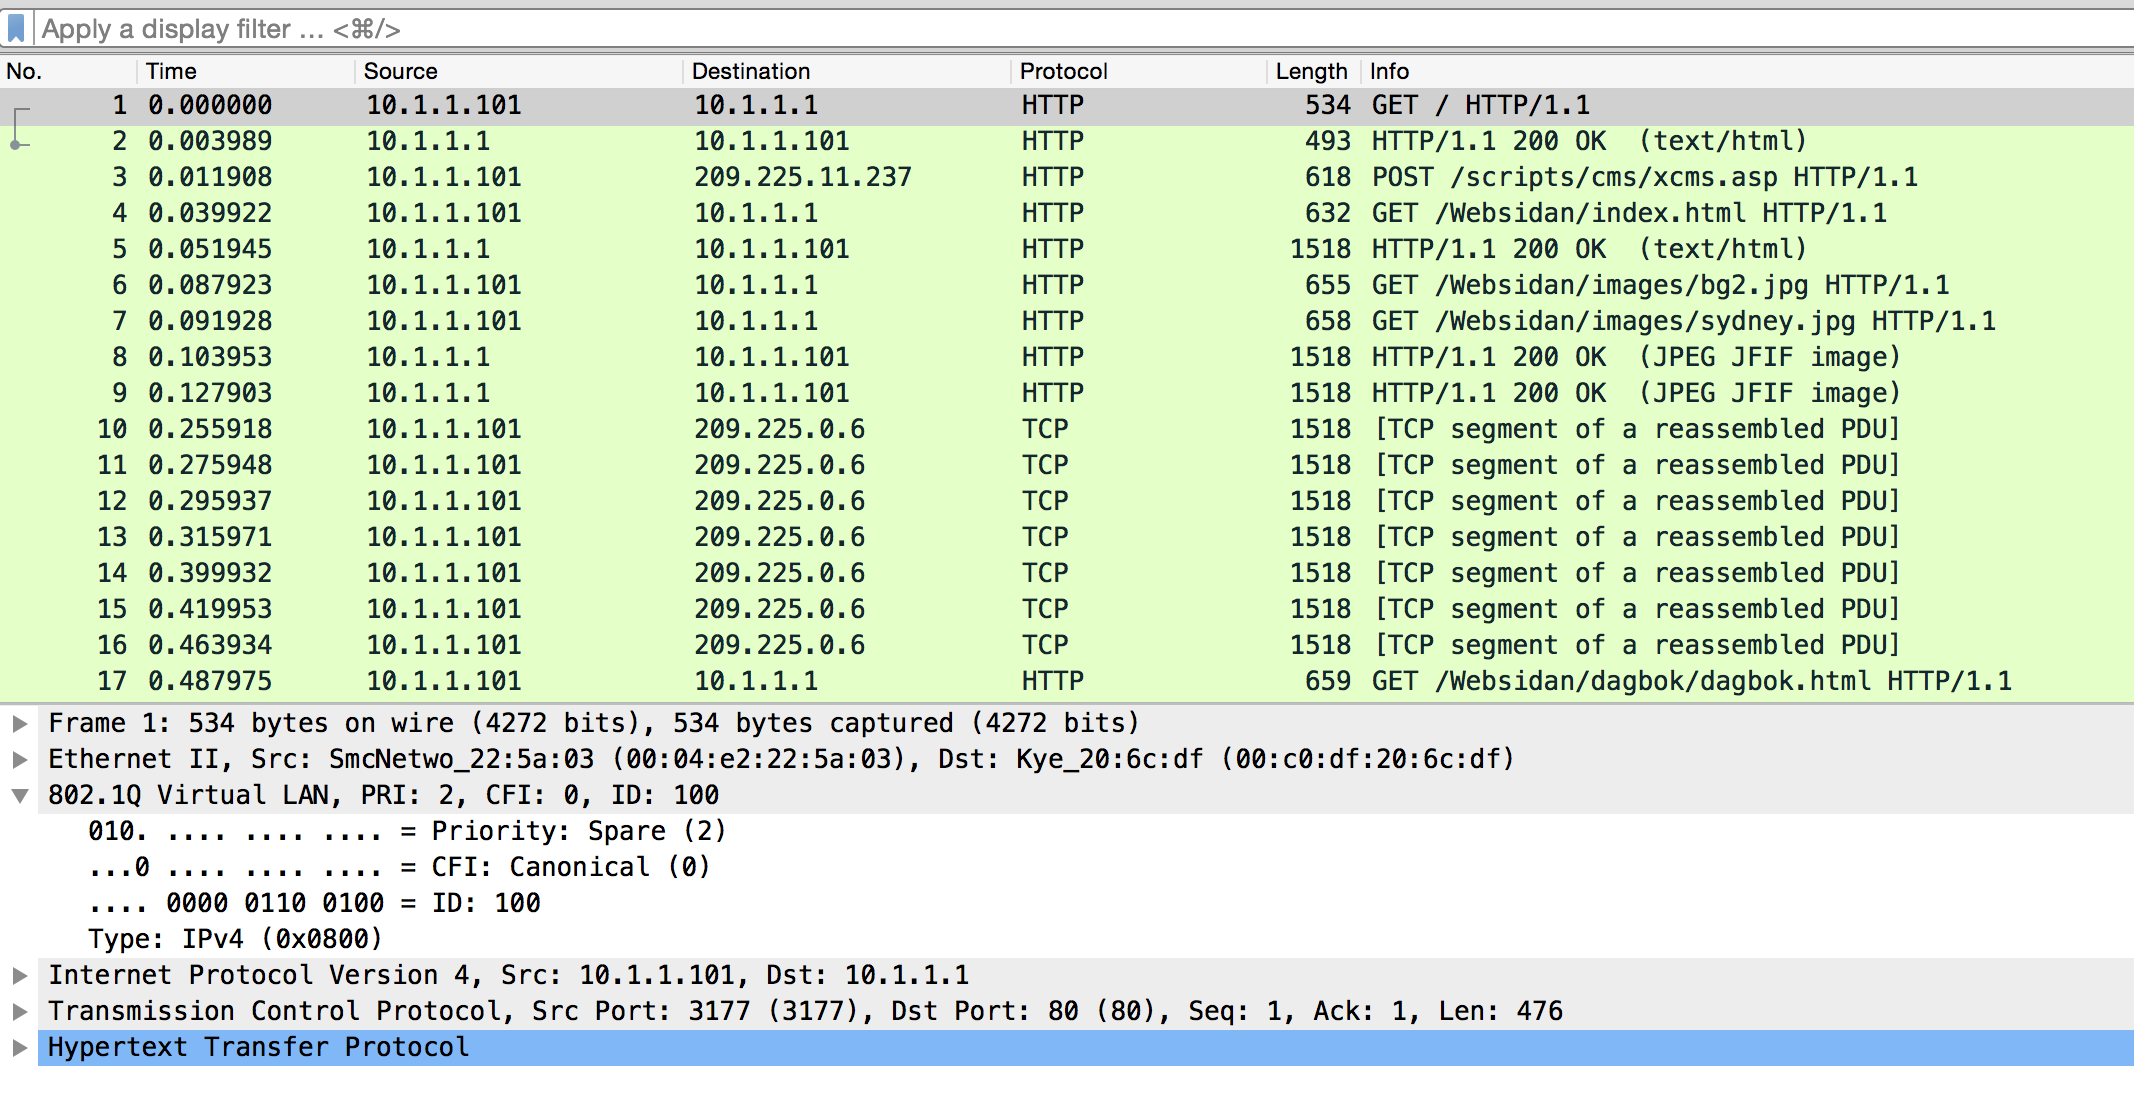
\includegraphics[scale=0.45]{pictures/wireshark}
\caption{Выходной трафик}
\label{pic:wireshark}
\end{figure}

Как видно на рисунке~\ref{pic:wireshark}, к пакету добавилась VLAN метка с содержимым, заданным в конфигурационном файле. Это позволяет сделать вывод о правильности функционирования разработанного сервиса.

\subsection{Нагрузочное тестирование}

\paragraph{Выводы}

В рамках данного раздела производится выбор операционной системы и языка программирования, приводится список дополнительных инструментов, использующихся при разработке, и команды для их установки из репозиториев Ubuntu. Также описываются классы, их назначение в рамках всей системы, и методы, использующиеся в работе сервиса. В конце раздела отражены результаты по каждому виду проведенного в рамках разработки тестирования.

\chapter{Организационно-экономический раздел}
Организация и планирование процесса разработки программного обеспечения предусматривает выполнение следующих задач:
\begin{enumerate}[1.]
\item формирование состава выполняемых работ и группировка их по стадиям разработки;
\item расчет трудоемкости выполнения работ;
\item расчет количества исполнителей;
\item построение сетевого графика;
\item разработка календарного графика работ;
\item Анализ структуры затрат проекта;
\item Оценка экономической целесообразности проекта;
\end{enumerate}

\section{Основные этапы разработки программного продукта}
Разработку программного продукта разбивают на следующие стадии в соответствии с ЕСПД ГОСТ 19102-77:
\begin{enumerate}[1.]
\item \textbf{Техническое задание.} Постановка задач. Определение пакета прикладных программ, состава и структуры информационной базы. Выбор языков программирования. Предварительный выбор методов выполнения работы. Разработка календарного плана выполнения работ.
\item \textbf{Эскизный проект.} Предварительная разработка структуры входных и выходных данных. Разработка общего описания алгоритмов решения задач. Разработка пояснительной записки. Согласование и утверждение эскизного проекта.
\item \textbf{Технический проект.} Разработка алгоритмов решения задач. Разработка пояснительной записки. Согласование и утверждение технического проекта. Разработка структуры программы. Разработка программной документации и передача ее для включения в технический проект. Внесение правок в структуры, анализ и определение формы представления входных и выходных данных. Выбор конфигурации технических средств.
\item \textbf{Рабочий проект.} Комплексная отладка задач и сдача в опытную эксплуатацию. Разработка проектной документации. Программирование и отладка программ. Описание контрольного примера. Разработка программной документации. 
\item \textbf{Внедрение.} Подготовка и передача программной документации для сопровождения с оформлением соответствующего акта. Передача программной продукции в фонд алгоритмов и программ. Проверка алгоритмов и программ решения задач, корректировка документации после опытной эксплуатации программного продукта.
\end{enumerate}

Анализируя требования ГОСТ, можно предложить следующее распределение работ по этапам:
\begin{enumerate}[1.]
\item Разработка технических требований, предъявляемых к разрабатываемому ПО и проведение исследований заданной области.
\item Разработка алгоритмов работы ПО, выбор среды программирования.
\item Разработка программных модулей (написание кода).
\item Тестирование и отладка разрабатываемого ПО.
\item Разработка документации.
\end{enumerate}

Этап внедрения отсутствует, так как разрабатываемое ПО будет внедряться силами заказчиков данного ПО без участия разработчиков.

\section{Расчет трудоемкости проекта}
Определим вероятные трудозатраты на выполнение данного проекта. Существует несколько методик опеределния трудозатрат, воспользуемся опеределением с помощью экспертных оценок. Для этой цели было опрошено четверо экспертов-разработчиков в области сетевых технологий.

В таблице~\ref{table:expert_marks} приведены оценки экспертов:

\begin{table}
\centering
\caption{Экспертные оценки}
\label{table:expert_marks}
\begin{tabular} {| c | c |} 
\hline
Эксперт 1 & 500\\
\hline
Эксперт 2 & 400\\
\hline
Эксперт 3 & 650\\
\hline
Эксперт 4 & 700\\
\hline
\end{tabular}
\end{table}

Общие затраты труда на разработку определим следующим образом:
\begin{equation}
Q_{P} = \sum_{i}t_i,
\end{equation}
где $t_{i}$ - затраты труда на выполнение i-го проекта.

Используя метод экспертных оценок, вычислим ожидаемую продолжительность работ T каждого этапа по формуле:
\begin{equation}
T = \frac{3 \cdot T_{MIN} + 2 \cdot T_{MAX}} {5} = \frac{3 \cdot 400 + 2 \cdot 700} {5} = 520,
\end{equation}
где $T_{MIN}$ - минимальная продолжительность работ, $T_{MAX}$ - максимальная продолжительность работ;

Продолжительности работ назначаются в соответствии с экспертными оценками, а ожидаемая продолжительность работы рассчитывается как математическое ожидание для $\beta$-распределения.

Полный перечень работ с разделением по этапам приведен в таблице~\ref{table:all_works}.
\begin{table}
\caption{Перечень работ}
\label{table:all_works}
\begin{tabular} {| p{0.15\textwidth} | p{0.08\textwidth} | p{0.3\textwidth} | p{0.1\textwidth} | p{0.1\textwidth} | p{0.1\textwidth} | p{0.09\textwidth} |} 
\hline
Этап & № & Содержание & $T_{MIN}$, & $T_{MAX}$, & T, & T, \\
& работы & работы & чел/часы & чел/часы & чел/часы & чел/дни\\
\hline
\multirow{4}{\hsize}{Разработка технических требований}
& 1 & Согласование списка поддерживаемых протоколов & 8 & 8 & 8 & 1\\
\cline{2-7}
& 2 & Разработка и утверждение ТЗ & 16 & 36 & 24 & 3\\
\cline{2-7}
& 3 & Анализ предметной области и существующих решений & 20 & 30 & 24 & 3\\
\cline{2-7}
& 4 & Анализ фреймворка DPDK и его возможностей & 16 & 16 & 16 & 2\\
\hline
\multirow{3}{\hsize}{Описание структур данных и алгоритмов}
& 5 & Разработка файла конфигурации: синтаксис, поддерживаемые действия, допустимые значения & 48 & 68 & 56 & 7\\
\cline{2-7}
& 6 & Разработка алгоритмов обнаружения протоколов & 72 & 92 & 80 & 10\\
\hline
\multirow{2}{\hsize}{Разработка программных модулей}
& 7 & Реализация модуля работы с файлом конфигурации & 60 & 70 & 64 & 8\\
\cline{2-7}
& 8 & Реализация главного модуля обработки сетевого трафика & 90 & 145 & 112 & 14\\
\hline
\multirow{3}{\hsize}{Тестирование и отладка ПО}
& 9 & Тестирование функциональности & 32 & 52 & 40 & 5\\
\cline{2-7}
& 10 & Тестирование производительности & 24 & 24 & 24 & 3 \\
\hline
Разработка документации & 12 & Написание программной и эксплуатационной документации & 66 & 81 & 72 & 9\\
\hline
\end{tabular}
\end{table}

Итого: $Q_{\textup{Р}} = Q_{\textup{ОЖ}} = 65 \textup{чел/дней} = 520 \textup{чел/час}$

\section{Определение численности исполнителей}
Средняя численность исполнителей определяется по формуле:
\begin{equation}
N = \frac{Q_{P}} {F},
\end{equation}
где F - фонд рабочего времени и определяется по формуле:
\begin{equation}
F = \sum_{i}^r F_{Mi} = \sum_{i}^r (D_{\textup{о}} - D{ \textup{в}} - D_{\textup{п}}),
\end{equation}
где $F_{Mi}$ - фонд времени в текущем i-том месяце и вычисляется для каждого месяца с учетом количества праздников $D_{\textup{о}}$, выходных $D_{\textup{в}}$ и праздничных $D_{\textup{п}}$ дней.

На реализацию проекта отведено r = 3 месяца рабочего времени при односменной работе с продолжительностью рабочего времени 8 часов. В таблице~\ref{table:time_fond} приведены сведения, необходимые для вычисления фонда времени для каждого месяца и итоговые результаты вычислений.
\begin{table}
\caption{Месячный фонд времени}
\label{table:time_fond}
\begin{tabular} {| p{0.1\textwidth} | p{0.2\textwidth} | p{0.15\textwidth} | p{0.15\textwidth} | p{0.15\textwidth} | p{0.15\textwidth} |} 
\hline
Месяц & Количество & Количество & Количество & Фонд & Фонд\\
& дней & выходных & праздничных & времени & времени \\
& & дней & дней & $F_{Mi}$,  дни & $F_{Mi}$, дни\\
\hline
Февраль & 29 & 8 & 1 & 20 & 159\\
\hline
Март & 31 & 9 & 1 & 21 & 168\\
\hline
Апрель & 30 & 9 & 0 & 21 & 168\\
\hline
Итого & & & & 62 & 495\\
\hline
\end{tabular}
\end{table}

Таким образом, фонд рабочего времени проекта составляет  F = 495 часов.

Отсюда средняя численность исполнителей равна:
\begin{equation}
N = \frac{Q_{P}} {F} = \frac{520} {495} = 1.05
\end{equation}

Таким образом, по суммарным трудозатратам для завершения проекта в заданные сроки необходимо два исполнителя: инженер и программист. Учитывая специфику дипломного проекта, данные специалисты должны обладать знаниями в следующих областях:
\begin{itemize}
\item протоколы вычислительных сетей;
\item сетевое программирование;
\item высокопроизводительные информационные системы и комплексы;
\item разработка алгоритмов и архитектуры ПО;
\item тестирование ПО;
\item разработка документации;
\end{itemize}

\section{Построение сетевого графика}
Для определения временных затрат и трудоемкости разработки ПО используем метод сетевого планирования. Этот метод позволяет установить единой схемой связь между всеми работами в виде наглядного и удобного для восприятия изображения (сетевого графика), представляющего собой информационно-динамическую модель, позволяющую определить продолжительность и трудоемкость как отдельных этапов, так и всего комплекса работ в целом.

Составление сетевой модели включает в себя оценку степени детализации комплекса работ и определения логической связи между отдельными работами. С этой целью составляется перечень всех основных работ и событий. В перечне указываются кодовые номера событий, наименования событий в последовательности от исходного к завершающему, кодовые номера работ, перечень всех работ, причем подряд указываются все работы, которые начинаются после наступления данного события.

Основные событий и работы представлены в таблице~\ref{table:events_and_works}.
\begin{longtable}{| p{0.03\textwidth} | p{0.33\textwidth} | p{0.1\textwidth} | p{0.3\textwidth} | p{0.07\textwidth} | p{0.07\textwidth} |} 
\caption{Основные работы и события проекта}
\label{table:events_and_works}
\\ \hline
$N_{i}$  & Наименование события & Код & Работа & t, & t,\\
& & работы & & чел/ч & чел/д \\
\hline \endfirsthead
\subcaption{Продолжение таблицы~\ref{table:events_and_works}}
\\ \hline \endhead
\hline \subcaption{Продолжение на след. стр.}
\endfoot
\hline \endlastfoot

0 & Разработка ПО начата & 0-1 & Согласование списка поддерживаемых протоколов & 8 & 1\\
\hline
1 & Протоколы согласованы & 1-2 & Разработка и утверждение ТЗ & 24 & 3\\
\hline
2 & ТЗ разработано и утверждено & 2-3 & Анализ предметной области и существующих решений & 24 & 3\\
\hline
3 & Анализ существующих решений проведен & 3-4 & Анализ фреймворка DPDK & 16 & 2\\
\hline
4 & DPDK проанализирован & 4-5 & Разработка файла конфигурации & 56 & 7\\
\cline{3-6}
& & 4-6 & Разработка алгоритмов обнаружения & 80 & 10\\
\hline
5 & Описание файла конфигурации выполнено & 5-6 & Фиктивная работа & 0 & 0\\
\hline
6 & Алгоритмы разработаны & 6-7 & Реализация модуля конфигурации & 64 & 8\\
\hline
7 & Модуль файла конфигурации реализован & 7-8 & Реализация главного модуля & 112 & 14\\
\hline
8 & Главный модуль реализован & 8-9 & Тестирование функциональности & 40 & 5\\
\cline{3-6}
& & 8-10 & Тестирование производительности & 24 & 3\\
\hline
9 & Функциональность протестирована & 9-11 & Разработка документации & 72 & 9\\
\hline
10 & Производительность протестирована & 10-12 & Фиктивная работа & 0 & 0\\
\hline
11 & Документация разработана & 11-12 & Фиктивная работа & 0 & 0\\
\hline
12 & Разработка ПО завершена & - & - & - & -\\

\end{longtable}

Сетевой график приведен на рисунке~\ref{fig:netgraph}.
\begin{figure}
\centering
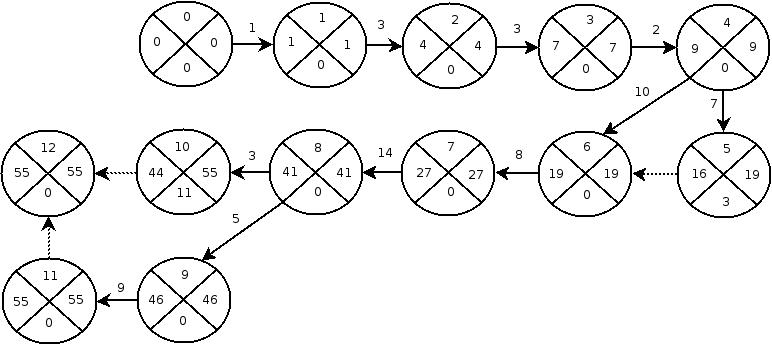
\includegraphics[scale=0.5]{pictures/netgraph}
\caption{Сетевой график}
\label{fig:netgraph}
\end{figure}

\section{Диаграмма Гантта}
Для иллюстрации последовательности проводимых работ на календарном графике приведена диаграмма Гантта (рисунок~\ref{fig:econom_gant}). По оси $X$ расположены календарные дни от начала проекта, а по оси $Y$ - выполняемые этапы работ.
\begin{figure}
\centering
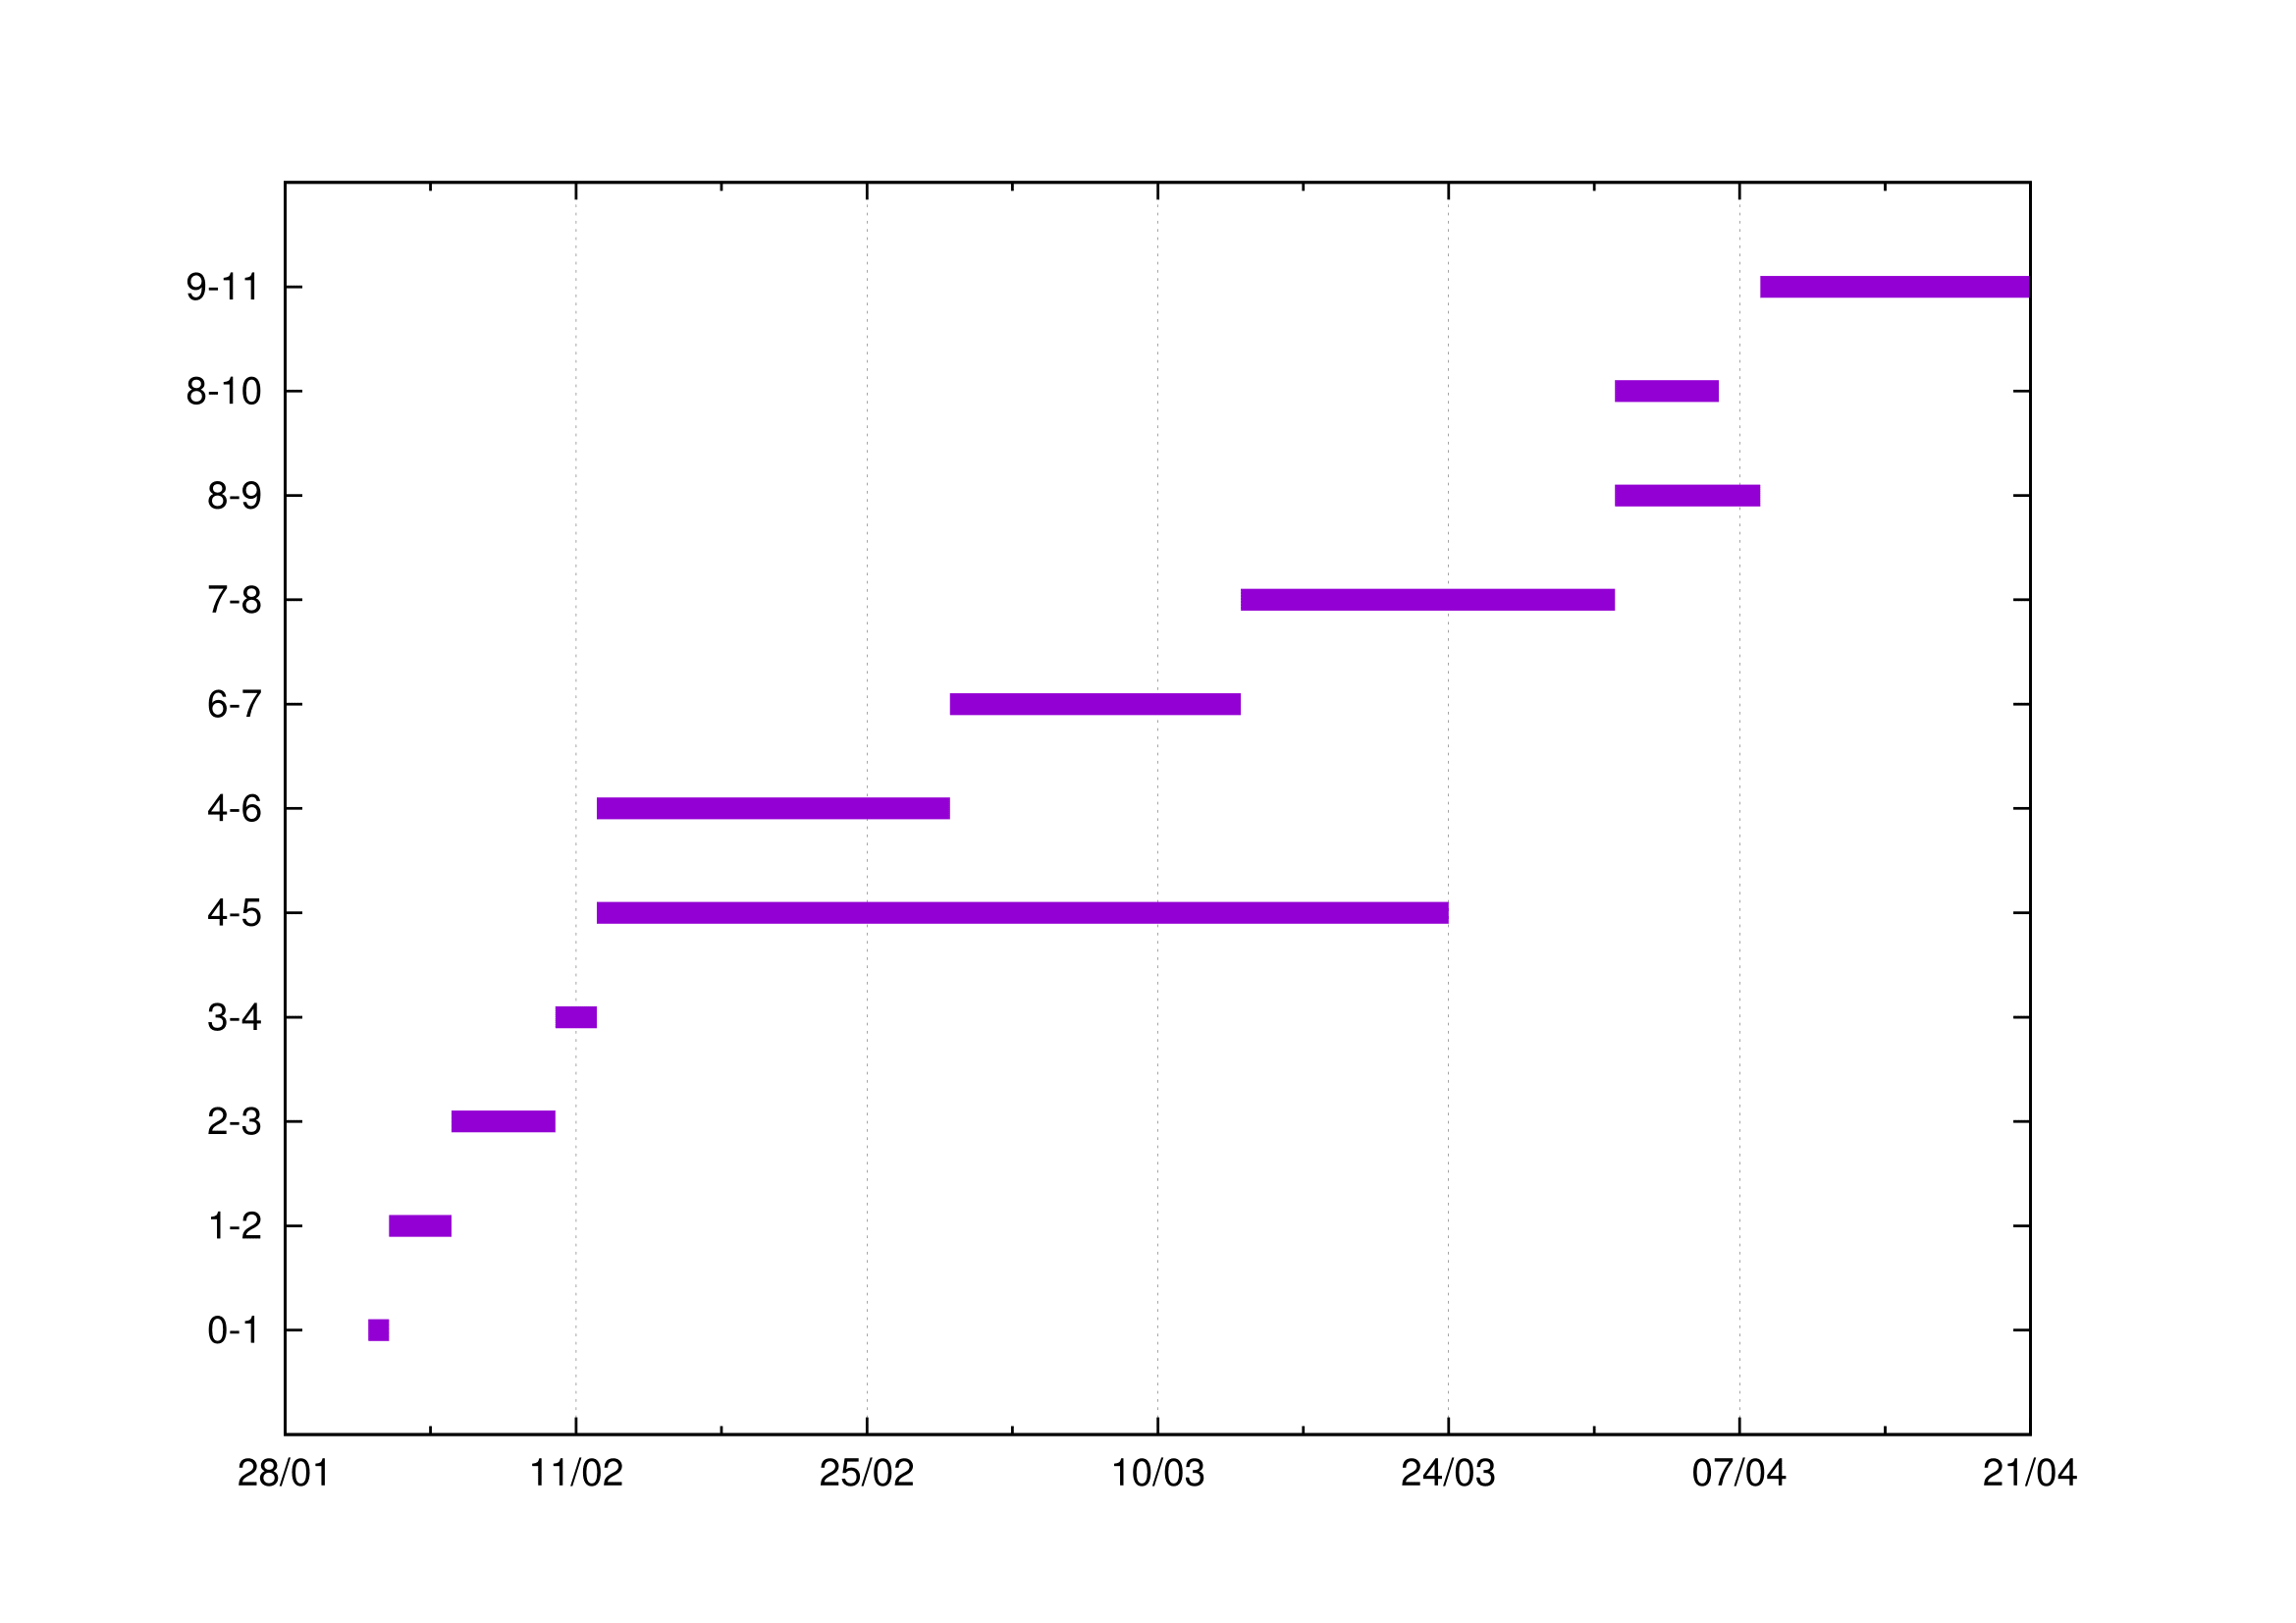
\includegraphics[scale=0.2]{pictures/gantt}
\caption{Диаграмма Гантта}
\label{fig:econom_gant}
\end{figure}

\begin{table}
\centering
\caption{Таблица занятости исполнителей}
\label{table:time_zan}
\begin{tabular} {| l | l | l | l |} 
\hline
Код работы &   Начало & Окончание & Исполнитель\\
\hline
0-1 & 02.02.16 & 02.02.16 & Программист\\
\hline
1-2 & 03.02.16 & 05.02.16 & Программист\\
\hline
2-3 & 08.02.16 & 10.02.16 & Программист\\
\hline
3-4 & 11.02.16 & 12.02.16 & Программист\\
\hline
4-5 & 15.02.16 & 24.03.16 & Программист\\
\hline
4-6 & 15.02.16 & 29.02.16 & Инженер\\
\hline
6-7 & 01.03.16 & 14.03.16 & Программист\\
\hline
7-8 & 15.03.16 & 01.04.16 & Программист\\
\hline
8-9 & 04.04.16 & 08.04.16 & Инженер\\
\hline
8-10 & 04.04.16 & 06.04.16 & Программист\\
\hline
9-11 & 11.04.16 & 21.04.16 & Инженер\\
\hline
\end{tabular}
\end{table}

\section{Анализ структуры и затрат проекта}
Затраты на выполнение проекта состоят из затрат на заработную плату исполнителям, затрат на закупку или аренду оборудования, затрат на организацию рабочих мест, и затрат на накладные раходы:
\begin{equation}
K = C_{\textup{ЗАРП}} + C_{\textup{ОБ}} + C_{\textup{ОРГ}} + C_{\textup{НАКЛ}},
\end{equation}
где $C_{\textup{ЗАРП}}$ - заработная плата исполнителей, $C_{\textup{ОБ}}$ - затраты на обеспечение необходимым оборудованием, $C_{\textup{ОРГ}}$ - затраты на организация рабочих мест, $C_{\textup{НАКЛ}}$ - накладные расходы.

\subsection{Затраты на выплату исполнителям заработной платы}
Затраты на выплату исполнителям заработной платы $C_{\textup{ЗАРП}}$ определяется следующим соотношением:
\begin{equation}
C_{\textup{ЗАРП}} = C_{\textup{З.ОСН}} + C_{\textup{З.ДОП}} + C_{\textup{З.ОТЧ}},
\end{equation}
где $C_{\textup{З.ОСН}}$ - основная заработная плата, $C_{\textup{З.ДОП}}$ - дополнительная заработная плата, $C_{\textup{З.ОТЧ}}$ - отчисления с заработной платы.

Расчет основной заработной платы при дневной оплате труда исполнителей проводится на основе данных по окладам и графику занятости исполнителей:
\begin{equation}
C_{\textup{З.ОСН}} = T_{\textup{ЗН}} \cdot O_{\textup{ДН}},
\end{equation}
где $O_{\textup{ДН}}$ - дневной оклад исполнителя, $T_{\textup{ЗН}}$ - число дней, отработанных исполнителем.

При 8-часовом рабочем дне $O_{\textup{ДН}}$ рассчитывается по формуле:
\begin{equation}
O_{\textup{ДН}} = \frac{O_{\textup{МЕС}} \cdot 8} {F_{M}},
\end{equation}
где $O_{\textup{МЕС}}$ - месячный оклад, $F_{M}$ - месячный фонд рабочего времени (приведен в таблице~\ref{table:time_fond}).

С учетом налога на доходы физических лиц размер месячного оклада увеличивается:
\begin{equation}
O_{\textup{МЕС}} = O \cdot (1 + \frac{H_{\textup{ДФЛ}}} {100}),
\end{equation}
где O - оклад, который позволит исполнителю заниматься проектом и который получен из информации кадровых агентств, $H_{\textup{ДФЛ}}$ - налог на доходы с физических лиц (13\%).

Предполагаемый размер заработной платы исполнителей был взят с интернет-портала www.hh.ru (03.05.2016). Расчет представлен в таблице~\ref{table:salary_of_executors} (размер оклада приведен с учетом налога на доходы с физических лиц).
\begin{table}
\caption{Оклады исполнителей}
\label{table:salary_of_executors}
\begin{tabular} {| l | l | l | l | l | l |} 
\hline
№ & Должность & "Чистый" & Дневной & Трудозатраты & Затраты на\\
&  & оклад, руб. & оклад, руб. & чел-день & зарплату, руб.\\
\hline
1 & Инженер & 100000 & 5478.79 & 24 & 131490.96\\
\hline
2 & Программист & 90000 & 4930.91 & 41 & 202167.31\\
\hline
3 & Итого & & & & 333658.27\\
\hline
\end{tabular}
\end{table}

Дополнительная заработная плата. Учитываются все выплаты непосредственным исполнителям за время, не проработанное на производстве, в том числе: оплата очередных отпусков, компенсации на недоиспользованный отпуск и др. Эти выплаты составляют 20\% от основной заработной платы:

$C_{\textup{З.ДОП}}$ = 0.2 $\cdot$ 333658.27 = 66731.6 руб.

Отчисления в пенсионный фонд, фонд социального страхования, занятости, на страховую медицины. Согласно нормативным документам, суммарные отчисления этой категории составляют 30\% от размеров заработной платы:

$C_{\textup{З.ОТЧ}}$ = (333658.27 + 66731.6) $\cdot$ 0.3 = 120116.96 руб.

\subsection{Затраты на оборудование}
Для организации рабочего процесса необходимо приобрести следующее:
%\item Ноутбук Asus K501Ux (58000 руб.)
%\item Ноутбук G50-80 (39000 руб.)
\begin{table}
\caption{Расходные материалы и оборудование}
\begin{tabular} {| l | l | l | l | l | l |} 
\hline
№ & Наименование & Ед. изм. & Кол-во & Цена за ед., руб. & Сумма\\
\hline
1 & Ноутбук Lenovo IdeaPad 100 15 & шт & 1 & 30000 & 30000\\
\hline
2 & Ноутбук Lenovo G50-80 & шт & 1 & 39000 & 39000\\
\hline
3 & Ручка шариковая синяя & шт & 4 & 68.50 & 274\\
& Pilot BPS-GP-EF & & & &\\
\hline
4 & Бумага Снегурочка & шт & 2 & 234 & 936\\
& (A4, 80 г/кв.м, белизна 146\% & & & &\\
& CIE, 500 листов) & & & &\\
\hline
5 & Итого & & & & 70210\\
\hline
\end{tabular}
\end{table}

\subsection{Расчет затрат, связанных с организацией рабочих мест}
Расчет затрат, связанных с организацией рабочих мест для исполнителей проекта, следует проводить ориентируясь на требования санитарных норм и правил, а также на стоимость аренды помещения требуемого уровня сервиса. В соответствии с санитарными нормами расстояние между рабочими столами с видеомониторами должно быть не менее 2 м., а между боковыми поверхностями видеомониторов - не менее 1.2 м.. Площадь на одно рабочее место с терминалом или ПК должна составлять не менее 6 кв.м., а объем - не менее 20 куб.м.. Расположение рабочих мест в подвальных помещениях не допускается. Помещения должны быть оборудованы системами отопления, кондиционирования воздуха или эффективной приточно-вытяжной системой.

Таким образом, необходимо подобрать рабочее помещение для рабочих мест двух исполнителей, что суммарно составляет не менее 12 кв.м..

В ходе исследования имеющихся предложений аренды офисных помещений были найдены варианты, приведенные в таблице~\ref{table:offices}.
\begin{table}[ht]
\caption{Офисные помещения}
\label{table:offices}
\begin{tabular} {| l | p{0.3\textwidth} | l | l | p{0.4\textwidth} |} 
\hline
№ & Адрес & Площадь & Стоимость  & Ссылка на сайт агенства\\
& & & кв.м./год & недвижимости\\
\hline
1 & Москва, Смольная ул, 24а & 16 & 14250 & http://irr.ru/real-estate/ commercial/offices/arenda-ofisa- 16-kv-m-m-vodnyy-stadion-advert551785147.html\\
\hline
2 & Москва, Черкизовская Б. ул & 15 & 13000 & http://irr.ru/real-estate/commer cial/offices/arenda-ofisov-pl- 15-275-m2-m-cherkizovskaya- v-advert551455572.html\\
\hline
3 & Москва, Докукина ул, 8с1 & 12 & 19833 & http://irr.ru/real-estate/ commercial/offices/arenda-ofisa- 11-9-kv-m-m- botanicheskiy-sad-advert551102848.html\\
\hline
4 & Москва, Шереметьевская ул, 47 & 13 & 14323 & http://irr.ru/real-estate/ commercial/offices/sdaetsya-ofis- 13-3-m2-m-mar-ina-roscha- advert550747753.html\\
\hline
\end{tabular}
\end{table}

Из таблицы~\ref{table:offices} следует, что наиболее выгодными является вариант 4, офисное помещение площадью 13 кв.м. в районе Марьина Роща г. Москвы.

Затраты на аренду помещения:

$C_{\textup{ОРГ}} = \frac{C_{\textup{КВМ}}} {12} \cdot S \cdot T_{\textup{АР}}$ = 46527 руб.

\subsection{Накладные расходы}
Накладные расходы состоят из расходов на производство, управление, техническое обслуживание и прочее. С учетом минимизации затрат, накладные расходы составляют 60\% от основной заработной платы:

$C_{\textup{НАКЛ}} = 0.6 \cdot C_{\textup{ОСН}} = 0.6 \cdot 333658.27$ = 200194.96 руб.

\subsection{Суммарные затраты}
Круговая диаграмма, отображающая структуру затрат проекта, приведена на рисунке~\ref{fig:circle_diagram}. Расчет суммарных затрат на реализацию программного проекта приведен в таблице~\ref{table:all_expenses}.

\begin{figure}
\centering
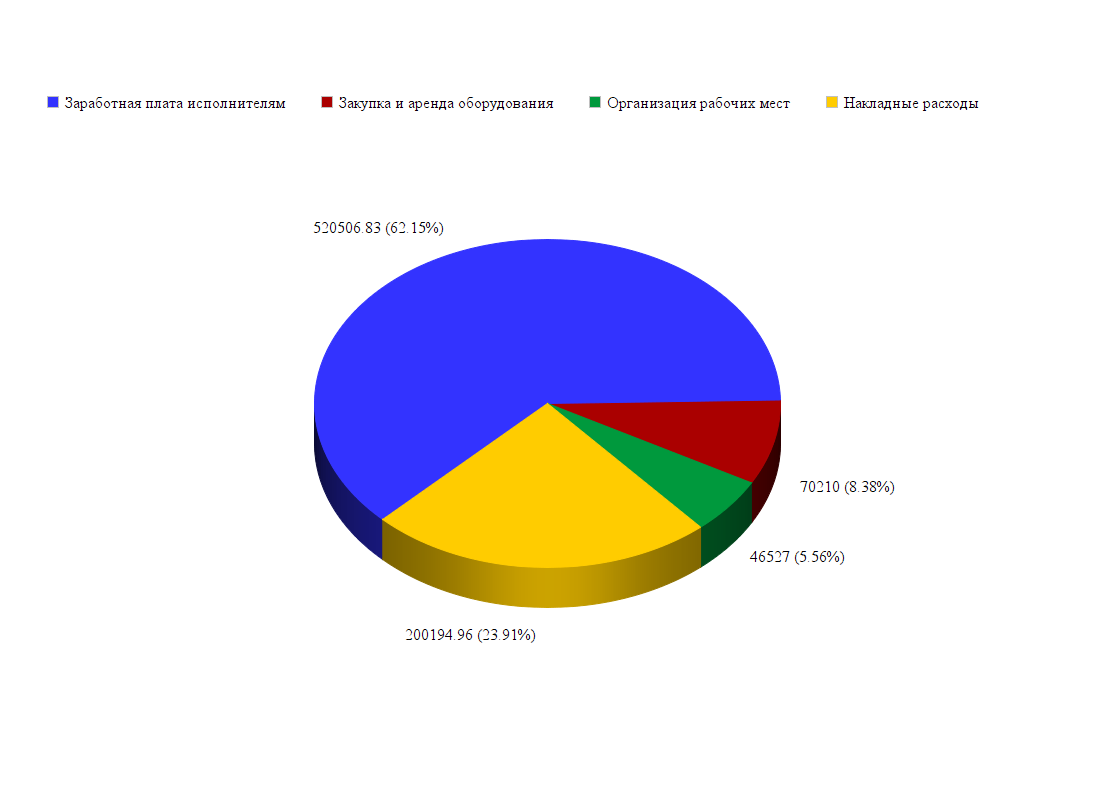
\includegraphics[scale=0.4]{pictures/circle_diagram}
\caption{Диаграмма затрат}
\label{fig:circle_diagram}
\end{figure}

\begin{table}
\caption{Суммарные затраты}
\label{table:all_expenses}
\begin{tabular} {| l | l | l | l |} 
\hline
№ & Статья расходов & Затраты, руб. & Доля, \%\\
\hline
1 &  Заработная плата исполнителям & 520506.83 & 62.15\\
\hline
2 & Закупка и аренда оборудования & 70210 & 8.38\\
\hline
3 & Организация рабочих мест & 46527 & 5.56\\
\hline
4 & Накладные расходы & 200194.96 & 23.91\\
\hline
5 & Итого & 837438.79 & 100\\
\hline
\end{tabular}
\end{table}


\section{Исследование рынка}
В разрабатываемом ПО в первую очередь заинтересованы операторы сотовых сетей и интернет-провайдеры, причем последние различных уровней, начиная от таких гигантов, как Ростелеком, оканчивая региональными филиалами.

Разрабатываемый продукт представляет собой сетевой сервис, позволяющий классифицировать трафик от L5 уровня сетевой модели и выше. Это, в свою очередь, позволяет эффективно управлять траффиком, блокировать его, настраивать сетевые экраны и т.д.

Предварительная оценка стоимости разрабатываемого ПО показала, что цена одного комплекта не будет превышать 30000 рублей.

Учитывая количество заинтересованных организаций только на территории Российской Федерации, оценим число потенциальных покупателей на годовом интервале времени $N_{P}^O$=100.


\section{Планирование цены и прогнозирование прибыли}
Частичная стоимость разработки, приходящаяся на каждый комплект ПО, определяется исходя из данных о планируемом объеме установок:
\begin{equation}
\Delta K = \frac{K} {N_{P}^O} \cdot (1+H_{\textup{СТ}}),
\end{equation}
где K - стоимость проекта, $N_{P}^O$ - планируемое число копий ПО, $H_{\textup{СТ}}$ - ставка банковского процента по долгосрочным кредитам (> 1 года).

Приняв ставку процента по долгосрочным кредитам за 24.9\% (ЗАО "Райфайзенбанк") и используя полученные ранее значения, вычислим:

$\Delta K = \frac{837438.79} {100} \cdot (1+0.249)$ = 10459.61 руб.

По результатам мониторинга рынка установим $K_{\textup{ПР}}$ = 30000 рублей. Тем самым, сумма от продаж за год составит 3000000 рублей, что обеспечит окупаемость проекта менее чем за 1 год. Определим процент прибыли от одной реализации ПО по формуле:
\begin{equation}
D_{\textup{ПРИБ}} = (\frac{K_{\textup{ПР}}} {\Delta K + K_{\textup{ВН} - 1}}) \cdot 100\%,
\end{equation}
где $K_{\textup{ВН}} = 0$ - затраты не внедрение.

Итого $D_{\textup{ПРИБ}} = 186.82\%$.

Сумма расчетной прибыли от продажи каждой установки ПО с учетом налога на добавочную стоимость $H_{\textup{НДС}} = 18\%$:
\begin{equation}
C_{\textup{ПРИБ}} = (\Delta K + K_{\textup{ВН}}) \cdot D_{\textup{ПРИБ}} \cdot (1 - H_{\textup{НДС}}) = 16023.33 руб.
\end{equation}

Для оплаты расходов на разработку ПО возьмем кредит в банке ЗАО "Райфайзенбанк" в размере 840000 рублей на срок 12 месяцев. Сумма погашения составляет 1049160 рублей. За первые 3 месяца разработки продажи равны нулю, т.к. продукт еще не разработан, при этом осуществляются выплаты заработной платы и производятся другие раннее рассчитанные расходы на разработку. В таблице~\ref{table:money_balance} приведен фрагмент общего баланса, из которого видно, что в сентябре 2016 года возможно досрочное погашение кредита.
\begin{table}
\caption{Фрагмент таблицы общего баланса}
\label{table:money_balance}
\begin{tabular} {| c | c | c | c | c | c | c |} 
\hline
Период & Баланс & Сумма & Сумма & Чистая & Баланс & Остаток\\
расчета & начальный, & продаж, & погашения & прибыль, & конечный, & по кредиту,\\
& руб & руб & кредита, руб & руб & руб & руб\\
\hline
02-04.2016 & 840000 & 0 & 262290 & -837438.79 & 2561.21 & 1049160.0\\
\hline
05.2016 & 2561.21 & 250000.0 & 87430.0 & 162570.0 & 165131.21 & 961730.0\\
\hline
06.2016 & 165131.21 & 250000.0 & 87430.0 & 162570.0 & 327701.21 & 874300.0\\
\hline
07.2016 & 327701.21 & 250000.0 & 87430.0 & 162570.0 & 490271.21 & 786870.0\\
\hline
08.2016 & 490271.21 & 250000.0 & 87430.0 & 162570.0 & 652841.21 & 699440.0\\
\hline
09.2016 & 652841.21 & 250000.0 & 87430.0 & 162570.0 & 815411.21 & 612010.0\\
\hline
\end{tabular}
\end{table}


\paragraph{Выводы}

Результаты проведенных организационно-экономических расчетов позволили оценить структуру работ и необходимое количество исполнителей. Общие затраты труда для выполнения проекта составили 65 чел/дней или 520 чел/часов. Затраты на разработку ПО составляют 837438.79 рублей.

Исходя из временных требований к реализации проекта, а также требований к квалификации персонала, была определена численность исполнителей: 2 человека - инженер и программист. По результатам построения сетевого графика и диаграммы Гантта можно сделать вывод о том, что введение дополнительных разработчиков не принесет положительного эффекта, а только увеличит затраты.

Из структуры затрат проекта видно, что основной статьей расходов является заработная плата исполнителей (62.15\%).

Для осуществления процесса разработки предполагается взять кредит в ЗАО "Райфайзенбанк" на срок 12 месяцев под 24.9\% годовых. Размер ежемесячного платежа по кредиту  составит 87430 рублей.

Стоимость 1 копии продукта составила 30000 рублей, при условии продажи 100 экземпляров в год. Планирование цены позволило спрогнозировать срок окупаемости проекта в пределах 1 года.

На основании вышеизложенного можно сделать вывод о том, что проект является экономически целесообразным.

\chapter{Охрана труда и экология}


\section{Анализ опасных и вредных факторов}
При работе на персональном компьютере пользователи подвергаются целому ряду вредных и опасных факторов, которые при несоблюдении установленных норм сказываются на здоровье человека отрицательным образом.

Документом, устанавливающим нормы воздействия вредных факторов при работе с видеодисплейными терминалами (ВДТ) и электронно-вычислительными машинами (ЭВМ), являются СанПиН 2.2.2/2.4.1340-03.

При создании данного программного  продукта использовался ноутбук Lenovo G50-80. Следовательно, согласно таблице 1 приложения 1 СанПиН 2.2.2/2.4.1340-03, требуется проконтролировать следующие параметры: уровень электромагнитных полей, уровень акустического шума, концентрацию вредных веществ в воздухе. Кроме этого следует учесть требования к помещениям, освещению и микроклимату.


\section{Освещение}
Наиболее важным условием эффективной работы программистов и пользователей является соблюдение оптимальных параметров системы освещения в рабочих помещениях.

Естественное освещение осуществляется через светопроемы, ориентированные в основном на север и северо-восток (для исключения попадания прямых солнечных лучей на экраны компьютеров) и обеспечивает коэффициент естественной освещенности (КЕО) не ниже 1,5\%.

В качестве искусственного освещения проектом предусмотрено использование системы общего равномерного освещения. В соответствии с СанПиН 2.2.2/2.4.1340-03 освещенность на поверхности рабочего стола находится в пределах 300-500 лк. Разрешается использование светильников местного освещения для работы с документами (при этом светильники не должны создавать блики на поверхности экрана).

Правильное расположение рабочих мест относительно источников освещения, отсутствие зеркальных поверхностей и использование матовых материалов ограничивает прямую (от источников освещения) и отраженную (от рабочих
поверхностей) блескость. При этом яркость светящихся поверхностей не превышает 200 кд/кв.м, яркость бликов на экране ПЭВМ не превышает 40 кд/кв.м, и яркость потолка не превышает 200 кд/кв.м.


\section{Напряжение в электрической сети}
Электрические установки, к которым относится практически все оборудование ЭВМ, представляют собой большую потенциальную опасность, поскольку в процессе эксплуатации или проведения профилактических работ человек может коснуться частей, находящихся под напряжением. Специфическая опасность электроустановок - токоведущие проводники, корпуса стоек ЭВМ и прочего оборудования, оказавшегося под напряжением в результате повреждения (пробоя) изоляции, не подают каких-либо сигналов, которые могли бы предупредить человека об опасности.

Помещение, в котором проводилась разработка, согласно ПУЭ, относится ко II-й категории - помещение с повышенной опасностью, напряжение в сети составляет 220 В, частота переменного тока - 50 Гц, поэтому для обеспечения безопасности использовались:
\begin{itemize}
\item Двойная изоляция проводников, сопротивление которой, согласно ПУЭ должно составлять 0.5 МОм;
\item Устройства аварийного отключения питания;
\end{itemize}


\section{Электрические и магнитные поля}
Большая часть составных частей ПЭВМ (системный блок, монитор, клавиатура, дисковые накопители, принтер, сканер) являются источником электромагнитных полей \cite{pc_izluch}. Примерные частоты электромагнитных полей (ЭМП), создаваемых различными устройствами приведены в таблице~\ref{table:ch_evm}.

\begin{table}
\caption{Частоты ЭМП, создаваемые различными устройствами ЭВМ}
\label{table:ch_evm}
\begin{tabular}{| p{0.5\textwidth} | p{0.5\textwidth} |}
\hline
Источник & Диапазон частот (первая гармоника)\\
\hline
Монитор & 50 Гц\\
\hline
Процессор & 50 Гц - 1000 МГц\\
\hline
Источник бесперебойного питания & 100 кГц\\
\hline
Другие устройства & 50 Гц\\
\hline
\end{tabular}
\end{table}

В таблице~\ref{table:vrur_evm} приводятся временные допустимые уровни ЭМП, создаваемых ЭВМ.

При разработке и использовании программного обеспечения предусматривается использование монитора (экран ноутбука), удовлетворяющего требованиям ТСО’06. Такие периферийные устройства, как принтер, не использовались.

\begin{table}[h]
\caption{Временные допустимые уровни ЭМП, создаваемые ЭВМ}
\label{table:vrur_evm}
\begin{tabular}{| p{0.4\textwidth} | p{0.3\textwidth} | p{0.2\textwidth} |}
\hline
Наименование параметров & \multicolumn{2}{l |}{ВДУ ЭМП}\\
\hline
Напряженность эл. поля & Диапазон 5 Гц - 2 кГц & 25 В/м\\
\cline{2-3}
& Диапазон 2 кГц - 400 кГц & 2.5 В/м\\
\hline
Плотность магнитного поля & Диапазон 5 Гц - 2 кГц & 250 нТл\\
\cline{2-3}
& Диапазон 2 кГц - 400 кГц & 25 нТл\\
\hline
\end{tabular}
\end{table}


\section{Шум и вибрация}
При постоянной работе на ЭВМ уровень вибрации не должен превышать допустимых норм вибрации. СанПиН 2.2.2/2.4.1340-03 устанавливает следующие предельно допустимые значения вибрации для рабочих мест (таблица~\ref{table:vibrac}).

\begin{table}[h]
\caption{Допустимые значения вибрации}
\label{table:vibrac}
\begin{tabular}{| p{0.5\textwidth} | l | l |}
\hline
\multirow{3}{\hsize}{Среднегеометрические частоты октавных полос, Гц}
& \multicolumn{2}{l |}{Допустимые значения}\\
\cline{2-3}
& \multicolumn{2}{l |}{по виброскорости}\\
\cline{2-3}
& м/c & дБ\\
\hline
2 & 4.5x10 & 79\\
\hline
4 & 2.2x10 & 73\\
\hline
8 & 1.1x10 & 67\\
\hline
16 & 1.1x10 & 67\\
\hline
31.5 & 1.1x10 & 67\\
\hline
63 & 1.1x10 & 67\\
\hline
Корректированные значения и их уровни, дБ & 2.0x10 & 72\\
\hline
\end{tabular}
\end{table}

К внутренним источникам шума относятся вентиляторы, принтеры и другие периферийные устройства ЭВМ. Мощные источники шума такие как сервера должны располагаться в отдельных помещениях с использованием средств звукоизоляции (звукопоглощающих материалов для облицовки стен и потолка помещения) и толстых перегородок (стен).

К внешним источникам шума можно отнести шум с улицы и соседних помещений. Для снижения шума улицы следует использовать более толстые шумопоглощающие стеклопакеты, а проветривание помещения осуществлять посредством системы кондиционирования. Для уменьшения шума соседних комнат следует использовать облицовку стен звукопоглощающими материалами.


\section{Микроклимат}
Согласно пункту 4.2 СанПиН 2.2.2/2.4.1340-03, в производственных помещениях, в которых работа с использованием ЭВМ является основной и связана с нервноэмоциональным напряжением, должны обеспечиваться оптимальные параметры микроклимата для категории работа 1а и 1б в соответствии с действующими санитарно-эпидемиологическими нормативами микроклимата производственных помещений.

Работа программиста проводится в сидячем положении и не требует физического напряжения (расход энергии не более 120 ккал/час), поэтому данный вид работ относится к категории 1а.

Кроме того, допустимые уровни положительных и отрицательных аэроионов в воздухе помещений, где расположены ЭВМ, должны соответствовать санитарно-эпидемиологическим нормам, приведенным в таблице~\ref{table:ioni}.

\begin{table}
\caption{Уровни положительных и отрицательных ионов}
\label{table:ioni}
\begin{tabular}{| l | l | l |}
\hline
\multirow{2}{*}{Уровни}
& \multicolumn{2}{l |}{Число ионов в 1 куб.см воздуха}\\
\cline{2-3}
& n+ & n-\\
\hline
Минимально необходимое & 400 & 600\\
\hline
Оптимальное & 1500-3000 & 3000-5000\\
\hline
Предельно-допустимые & 50000 & 50000\\
\hline
\end{tabular}
\end{table}

Для поддержания уровней в пределах допустимых используются различные системы ионизации воздуха. Помещение, в котором проводились работы, оснащено общеобменной приточно-вытяжной системой вентиляции и биполярным ионизатором воздуха Янтарь-5А, рекомендованные для использования в жилых помещениях. Таким образом, параметры микроклимата и уровни ионизации воздуха в помещении приведены в соответствие с нормой (таблица~\ref{table:microclim}).

\begin{table}[h]
\caption{Параметры микроклимата}
\label{table:microclim}
\begin{tabular}{| p{0.2\textwidth} | p{0.2\textwidth} | p{0.3\textwidth} | p{0.25\textwidth} |}
\hline
Период года & \multicolumn{3}{c |}{Параметры}\\
\hline
& Температура воздуха, \textdegree C & Относительная влажность воздуха, \% & Скорость движения воздуха (не более), м/с\\
\hline
\multirow{1}{*}{Холодный}
& 22-24 & 40-60 & 0.1\\
\hline
\multirow{1}{*}{Теплый}
& 23-25 & 40-60 & 0.1\\
\hline
\end{tabular}
\end{table}


\section{Расчет уровня шума в серверной комнате}
Проведем расчет уровня звукового давления при заданном уровне звуковой мощности источника (таблица~\ref{table:level_sound_power}) в серверной комнате объемом 10x3x2, который расположен на полу на расстоянии 8 метров от расчетной точки.
\begin{table}[h]
\caption{Уровни звукового давления источника}
\label{table:level_sound_power}
\begin{tabular}{| l | l | l | l | l | l | l | l | l |}
\hline
Расстояние & \multicolumn{8}{c |}{Уровни звуковой мощности, дБ}\\
\cline{2-9}
до источника & 63 & 125 & 250 & 500 & 1000 & 2000 & 4000 & 8000\\
\hline
8 & 84 & 82 & 84 & 91 & 94 & 94 & 91 & 91\\
\hline
\end{tabular}
\end{table}

Ожидаемый уровень звукового давления в помещении можно вычислить по формуле \cite{bzd_book}:
\begin{equation}
L = L_{W} + 10 \cdot \lg(\frac{1}{2\pi R^2} + \frac{4}{m*V}),
\end{equation}
где $L_{W}$ - октавный уровень звуковой мощности источника шума, R - расстояние до источника, V - объем помещения, m - частотный множитель, зависящий от объема помещения и среднегеометрической частоты \cite{noise_book}.

Объем помещения составляет 60 $\textup{м}^3$, исходя из этого в таблице~\ref{table:m_values} приведены значения частотного множителя.
\begin{table}
\caption{Значения частотного множителя}
\label{table:m_values}
\begin{tabular}{| l | l | l | l | l | l | l | l |}
\hline
\multicolumn{8}{| c |}{Среднегеометрическая частота, Гц}\\
\hline
63 & 125 & 250 & 500 & 1000 & 2000 & 4000 & 8000\\
\hline
0.8 & 0.75 & 0.7 & 0.8 & 1.0 & 1.4 & 1.8 & 2.5\\
\hline
\end{tabular}
\end{table}

Результаты вычислений и нормативные значения уровней звукового давления приведены в таблице~\ref{table:noise_results}.
\begin{table}
\caption{Уровни звукового давления}
\label{table:noise_results}
\begin{tabular}{| l | l | l | l | l | l | l | l | l |}
\hline
\multirow{2}{*}{}
&\multicolumn{8}{c |}{Уровни звукового давления, дБ}\\
\cline{2-9}
& 63 & 125 & 250 & 500 & 1000 & 2000 & 4000 & 8000\\
\hline
$L$ & 73.34 & 71.60 & 73.90 & 80.34 & 82.40 & 81.00 & 76.97 & 75.65\\
\hline
$L_{lim}$ & 71 & 61 & 54 & 49 & 45 & 42 & 40 & 38\\
\hline
\end{tabular}
\end{table}

Полученные при расчете уровни шума для заданного помещения превышают предельно допустимые величины. Так как увеличение расстояния от источника до расчетной точки слабо влияет на уровень шума, а изменение размеров комнаты не снижает уровень шума до допустимых значений, рекомендуется использовать дополнительные методы борьбы с шумом такие как звукоизоляция. Звукоизоляция помещения осуществляется посредством звукоизолирующих материалов, облицовки стен, кожухов и кабин, заполнением воздушного пространства в двойных легких перегородках звукопоглощающими материалами, повышением воздухонепроницаемости преграды или применением экранов.

Так как уровни шума превышают допустимые уровни шума, то программисты не должны работать в данном помещении, а во время нахождения рядом с серверами следует использовать индивидуальные средства защиты (например, беруши).


\section{Утилизация компонентов ЭВМ}
Разрабатываемое программное обеспечение будет использоваться на мощных ЭВМ или серверах. По этой причине встает вопрос о правильной утилизации устаревшего оборудования.

Наибольшую ценность представляют собой различные платы, входящие в состав ЭВМ. В состав утилизированных отходов входят только те платы, которые содержат драгоценные металлы \cite[стр.~153]{utilization}. В современном понимании утилизация отходов представляет собой восстановление ценных материалов путем плавления металлического содержимого, однако стоимость этого процесса такова, что в переработку поступают только платы с очень высоким содержанием драгоценных металлов. Платы, поступающие в переплавку, все без исключения подвергаются обогащению посредством измельчения, а также магнитной и другой дополнительной классификации. Часть отходов, для захоронения которых могла бы понадобиться мусорная свалка, отправляются в Китай для разборки и пиролиза.

Обычно при утилизации используют следующие технологические маршруты:
\begin{itemize}
\item повторное использование компонентов путем их демонтажа;
\item восстановление материалов посредством их механической переработки, пирометаллургии, гидрометаллургии или сочетанием этих технологий;
\end{itemize}

Бракованные платы, отправляемые в плавильную печь, редко подвергаются какой-либо форме обогащения. Производятся только выборочный демонтаж, сортировка и измельчение демонтированных плат. Компании, занимающиеся утилизацией отходов электроники, довольно часто теряют примерно 10\% драгоценных драгоценных металлов, даже применяя процессы флотационного разделения. Потери при переработке плат, содержащих драгоценные металлы в компонентах, составляют примерно 35\%. Известно, что драгоценные металлы в основном присутствуют на выводах компонентов и на контактных площадках плат.

В США и Европе существуют специальные рынки, где продаются демонтированные и восстановленные компоненты плат. Они поступают на рынок с производств, где используют робототехнические системы, обеспечивающие возможность идентификации и демонтажа только тех компонентов, которых не достает на складе. Однако приходится считаться с тем, что быстрое обновление элементной базы и относительно низкая стоимость новых компонентов приведут к серьезному ограничению повторного использования демонтированных компонентов неопределенной давности.

Пиролитическая обработка обычно включает сжигание и плавление размельченного сырья при температуре примерно 1200 \textdegree C. Для этого требуется небольшое количество мазута, так как большая часть энергии обеспечивается за счет сгорания органических компонентов. При этой температуре сгорают органические составляющие отходов, а образующие дымы направляются в камеру дожигания, где они теряют свою токсичность при температуре 1400 \textdegree C. Остающийся от сжигания конгломерат называется "черным металлом". Он, как правило, представляет собой продукт богатый медью. Последующая электролитическая очистка и химическая обработка анодного осадка отделяет медь и другие компоненты от драгоценных металлов.

Новые технологии позволяют не сжигать, а перерабатывать пустые платы в изделия. Например, фирма, FUBA (Германия) перевела на коммерческую основу выделение от 92\% до 95\% металлов из отходов пустых печатных плат за счет использования механических и гидрометаллургических методов разделения. Они включают измельчение, гранулирование, магнитное разделение, классификацию и электростатическое разделение. Совокупность композиций, получаемая от этой обработки, нашла свое применение в изготовлении изделий, имеющих в своем составе большое количество стекловолокна, а также в качестве накопителей в производстве строительных материалов. Особенно успешным оказалось применение стеклополимерных композиций для производства емкостей и поддонов, стойких к химическому воздействию. Металлические составляющие отходов печатных плат (в основном медь) растворяются в таких выщелачивателях, как серная и азотная кислоты, с последующим электростатическим восстановлением меди.

Бракованные печатные платы обычно сортируют по трем категориям, которые отражают количество содержащихся в них драгоценны металлов. Это следующие категории: H - отходы с высоким содержанием драгоценных металлов, M - отходы со средним содержанием и L - отходы с низким содержанием драгметаллов. К H категории относятся дискретные компоненты, интегральные схемы, содержащие золото, устройства оптоэлектроники, платы с содержанием драгоценных металлов, с золоченными и паладированными контактами. Бракованные платы с компонентами по большей части вывозятся в Китай для повторного использования.

Таким образом, процесс утилизации и переработки плат является актуальной темой, а учитывая то, что в состав плат входят драгоценные металлы - является коммерчески выгодным. Это привело к развитию коммерческой инфраструктуры, основанной на сборе печатных плат с последующей их сортировкой по содержанию драгметаллов и восстановлением путем переплавки в плавильной печи. Также появляются новые методы обработки, призванные заменить устаревшие за счет большей эффективности и более дешевой эксплуатации.


\backmatter %% Здесь заканчивается нумерованная часть документа и начинаются ссылки и
            %% заключение

\Conclusion
В ходе выполнения дипломной работы были получены следующие результаты:
\begin{enumerate}[1.]
\item Проанализированы проблемы, с которыми сталкиваются интернет-провайдеры, а также предложены варианты их решения с использованием технологии DPI. Вместе с этим были рассмотрены наиболее популярные фреймворки быстрой обработки пакетов, выявлены их достоинства и недостатки. Разработана концептуальная модель сервиса.
\item Изучены протоколы HTTP, SIP, RTSP и RTP. На основе структуры данных протоколов разработаны алгоритмы обнаружения каждого из них.
\item Сформулирован список программного обеспечения, необходимый для полноценного функционирования сервиса. Приведены примеры команд для установки на Ubuntu.
\item Разработан сетевой сервис классификации трафика на основе технологии DPI, акселерированный DPDK. Проведено модульное, функциональное и нагрузочное тестирование данного сервиса.
\end{enumerate}



% % Список литературы при помощи BibTeX
% Юзать так:
%
% pdflatex rpz
% bibtex rpz
% pdflatex rpz

\bibliographystyle{gost780u}
\bibliography{rpz}

%%% Local Variables: 
%%% mode: latex
%%% TeX-master: "rpz"
%%% End: 


%\appendix   % Тут идут приложения
%\chapter{Картинки}
\label{cha:appendix1}

\begin{figure}
\centering
\caption{Картинка в приложении. Страшная и ужасная.}
\end{figure}

%%% Local Variables: 
%%% mode: latex
%%% TeX-master: "rpz"
%%% End: 

%\chapter{Еще картинки}
\label{cha:appendix2}

\begin{figure}
\centering
\caption{Еще одна картинка, ничем не лучше предыдущей. Но надо же как-то заполнить место.}
\end{figure}

%%% Local Variables: 
%%% mode: latex
%%% TeX-master: "rpz"
%%% End: 


\end{document}
